\documentclass[]{book}
\usepackage{lmodern}
\usepackage{amssymb,amsmath}
\usepackage{ifxetex,ifluatex}
\usepackage{fixltx2e} % provides \textsubscript
\ifnum 0\ifxetex 1\fi\ifluatex 1\fi=0 % if pdftex
  \usepackage[T1]{fontenc}
  \usepackage[utf8]{inputenc}
\else % if luatex or xelatex
  \ifxetex
    \usepackage{mathspec}
  \else
    \usepackage{fontspec}
  \fi
  \defaultfontfeatures{Ligatures=TeX,Scale=MatchLowercase}
\fi
% use upquote if available, for straight quotes in verbatim environments
\IfFileExists{upquote.sty}{\usepackage{upquote}}{}
% use microtype if available
\IfFileExists{microtype.sty}{%
\usepackage{microtype}
\UseMicrotypeSet[protrusion]{basicmath} % disable protrusion for tt fonts
}{}
\usepackage[margin=1in]{geometry}
\usepackage{hyperref}
\hypersetup{unicode=true,
            pdftitle={From Novice to Expert in Bioinformatics},
            pdfauthor={Shaojun Xie},
            pdfborder={0 0 0},
            breaklinks=true}
\urlstyle{same}  % don't use monospace font for urls
\usepackage{natbib}
\bibliographystyle{apalike}
\usepackage{color}
\usepackage{fancyvrb}
\newcommand{\VerbBar}{|}
\newcommand{\VERB}{\Verb[commandchars=\\\{\}]}
\DefineVerbatimEnvironment{Highlighting}{Verbatim}{commandchars=\\\{\}}
% Add ',fontsize=\small' for more characters per line
\usepackage{framed}
\definecolor{shadecolor}{RGB}{248,248,248}
\newenvironment{Shaded}{\begin{snugshade}}{\end{snugshade}}
\newcommand{\KeywordTok}[1]{\textcolor[rgb]{0.13,0.29,0.53}{\textbf{#1}}}
\newcommand{\DataTypeTok}[1]{\textcolor[rgb]{0.13,0.29,0.53}{#1}}
\newcommand{\DecValTok}[1]{\textcolor[rgb]{0.00,0.00,0.81}{#1}}
\newcommand{\BaseNTok}[1]{\textcolor[rgb]{0.00,0.00,0.81}{#1}}
\newcommand{\FloatTok}[1]{\textcolor[rgb]{0.00,0.00,0.81}{#1}}
\newcommand{\ConstantTok}[1]{\textcolor[rgb]{0.00,0.00,0.00}{#1}}
\newcommand{\CharTok}[1]{\textcolor[rgb]{0.31,0.60,0.02}{#1}}
\newcommand{\SpecialCharTok}[1]{\textcolor[rgb]{0.00,0.00,0.00}{#1}}
\newcommand{\StringTok}[1]{\textcolor[rgb]{0.31,0.60,0.02}{#1}}
\newcommand{\VerbatimStringTok}[1]{\textcolor[rgb]{0.31,0.60,0.02}{#1}}
\newcommand{\SpecialStringTok}[1]{\textcolor[rgb]{0.31,0.60,0.02}{#1}}
\newcommand{\ImportTok}[1]{#1}
\newcommand{\CommentTok}[1]{\textcolor[rgb]{0.56,0.35,0.01}{\textit{#1}}}
\newcommand{\DocumentationTok}[1]{\textcolor[rgb]{0.56,0.35,0.01}{\textbf{\textit{#1}}}}
\newcommand{\AnnotationTok}[1]{\textcolor[rgb]{0.56,0.35,0.01}{\textbf{\textit{#1}}}}
\newcommand{\CommentVarTok}[1]{\textcolor[rgb]{0.56,0.35,0.01}{\textbf{\textit{#1}}}}
\newcommand{\OtherTok}[1]{\textcolor[rgb]{0.56,0.35,0.01}{#1}}
\newcommand{\FunctionTok}[1]{\textcolor[rgb]{0.00,0.00,0.00}{#1}}
\newcommand{\VariableTok}[1]{\textcolor[rgb]{0.00,0.00,0.00}{#1}}
\newcommand{\ControlFlowTok}[1]{\textcolor[rgb]{0.13,0.29,0.53}{\textbf{#1}}}
\newcommand{\OperatorTok}[1]{\textcolor[rgb]{0.81,0.36,0.00}{\textbf{#1}}}
\newcommand{\BuiltInTok}[1]{#1}
\newcommand{\ExtensionTok}[1]{#1}
\newcommand{\PreprocessorTok}[1]{\textcolor[rgb]{0.56,0.35,0.01}{\textit{#1}}}
\newcommand{\AttributeTok}[1]{\textcolor[rgb]{0.77,0.63,0.00}{#1}}
\newcommand{\RegionMarkerTok}[1]{#1}
\newcommand{\InformationTok}[1]{\textcolor[rgb]{0.56,0.35,0.01}{\textbf{\textit{#1}}}}
\newcommand{\WarningTok}[1]{\textcolor[rgb]{0.56,0.35,0.01}{\textbf{\textit{#1}}}}
\newcommand{\AlertTok}[1]{\textcolor[rgb]{0.94,0.16,0.16}{#1}}
\newcommand{\ErrorTok}[1]{\textcolor[rgb]{0.64,0.00,0.00}{\textbf{#1}}}
\newcommand{\NormalTok}[1]{#1}
\usepackage{longtable,booktabs}
\usepackage{graphicx,grffile}
\makeatletter
\def\maxwidth{\ifdim\Gin@nat@width>\linewidth\linewidth\else\Gin@nat@width\fi}
\def\maxheight{\ifdim\Gin@nat@height>\textheight\textheight\else\Gin@nat@height\fi}
\makeatother
% Scale images if necessary, so that they will not overflow the page
% margins by default, and it is still possible to overwrite the defaults
% using explicit options in \includegraphics[width, height, ...]{}
\setkeys{Gin}{width=\maxwidth,height=\maxheight,keepaspectratio}
\IfFileExists{parskip.sty}{%
\usepackage{parskip}
}{% else
\setlength{\parindent}{0pt}
\setlength{\parskip}{6pt plus 2pt minus 1pt}
}
\setlength{\emergencystretch}{3em}  % prevent overfull lines
\providecommand{\tightlist}{%
  \setlength{\itemsep}{0pt}\setlength{\parskip}{0pt}}
\setcounter{secnumdepth}{5}
% Redefines (sub)paragraphs to behave more like sections
\ifx\paragraph\undefined\else
\let\oldparagraph\paragraph
\renewcommand{\paragraph}[1]{\oldparagraph{#1}\mbox{}}
\fi
\ifx\subparagraph\undefined\else
\let\oldsubparagraph\subparagraph
\renewcommand{\subparagraph}[1]{\oldsubparagraph{#1}\mbox{}}
\fi

%%% Use protect on footnotes to avoid problems with footnotes in titles
\let\rmarkdownfootnote\footnote%
\def\footnote{\protect\rmarkdownfootnote}

%%% Change title format to be more compact
\usepackage{titling}

% Create subtitle command for use in maketitle
\newcommand{\subtitle}[1]{
  \posttitle{
    \begin{center}\large#1\end{center}
    }
}

\setlength{\droptitle}{-2em}
  \title{From Novice to Expert in Bioinformatics}
  \pretitle{\vspace{\droptitle}\centering\huge}
  \posttitle{\par}
\subtitle{Linux, Perl and R for Bioinformatics}
  \author{Shaojun Xie}
  \preauthor{\centering\large\emph}
  \postauthor{\par}
  \predate{\centering\large\emph}
  \postdate{\par}
  \date{2017-11-07}

\usepackage{booktabs}

\makeatletter
\newenvironment{kframe}{%
\medskip{}
\setlength{\fboxsep}{.8em}
 \def\at@end@of@kframe{}%
 \ifinner\ifhmode%
  \def\at@end@of@kframe{\end{minipage}}%
  \begin{minipage}{\columnwidth}%
 \fi\fi%
 \def\FrameCommand##1{\hskip\@totalleftmargin \hskip-\fboxsep
 \colorbox{shadecolor}{##1}\hskip-\fboxsep
     % There is no \\@totalrightmargin, so:
     \hskip-\linewidth \hskip-\@totalleftmargin \hskip\columnwidth}%
 \MakeFramed {\advance\hsize-\width
   \@totalleftmargin\z@ \linewidth\hsize
   \@setminipage}}%
 {\par\unskip\endMakeFramed%
 \at@end@of@kframe}
\makeatother

\renewenvironment{Shaded}{\begin{kframe}}{\end{kframe}}

\newenvironment{rmdblock}[1]
  {
  \begin{itemize}
  \renewcommand{\labelitemi}{
    \raisebox{-.7\height}[0pt][0pt]{
      {\setkeys{Gin}{width=3em,keepaspectratio}\includegraphics{images/#1}}
    }
  }
  \setlength{\fboxsep}{1em}
  \begin{kframe}
  \item
  }
  {
  \end{kframe}
  \end{itemize}
  }
\newenvironment{rmdnote}
  {\begin{rmdblock}{note}}
  {\end{rmdblock}}
\newenvironment{rmdcaution}
  {\begin{rmdblock}{caution}}
  {\end{rmdblock}}
\newenvironment{rmdimportant}
  {\begin{rmdblock}{important}}
  {\end{rmdblock}}
\newenvironment{rmdtip}
  {\begin{rmdblock}{tip}}
  {\end{rmdblock}}
\newenvironment{rmdwarning}
  {\begin{rmdblock}{warning}}
  {\end{rmdblock}}

\usepackage{amsthm}
\newtheorem{theorem}{Theorem}[chapter]
\newtheorem{lemma}{Lemma}[chapter]
\theoremstyle{definition}
\newtheorem{definition}{Definition}[chapter]
\newtheorem{corollary}{Corollary}[chapter]
\newtheorem{proposition}{Proposition}[chapter]
\theoremstyle{definition}
\newtheorem{example}{Example}[chapter]
\theoremstyle{definition}
\newtheorem{exercise}{Exercise}[chapter]
\theoremstyle{remark}
\newtheorem*{remark}{Remark}
\newtheorem*{solution}{Solution}
\let\BeginKnitrBlock\begin \let\EndKnitrBlock\end
\begin{document}
\maketitle

{
\setcounter{tocdepth}{1}
\tableofcontents
}
\chapter*{Preface}\label{preface}
\addcontentsline{toc}{chapter}{Preface}

\section*{Who should read this book?}\label{who-should-read-this-book}
\addcontentsline{toc}{section}{Who should read this book?}

I started to do NGS data analysis as a bench researcher. I started from
ZERO. I understand how people feel when they were ZERO. So this book is
written for researchers who have no prior knowledge of NGS data
analysis. You do NOT need any programming background. If you already
have some, that's good. All you need is the strength and the resolution
to finish this book.

For those of you who already have some experience but you still don't
feel comfortable when dealing with the data, this will be for you. In
this book, I will write some skills that I have learned, which will
accelerate your analysis.

\section*{How to read this book?}\label{how-to-read-this-book}
\addcontentsline{toc}{section}{How to read this book?}

This is not a sci-fiction books. This is a technical book. I highly
recommend you to practice when you're reading this book.

\emph{\textbf{Don't panic!}}

\section*{The reason why I didn't write in
Chinese?}\label{the-reason-why-i-didnt-write-in-chinese}
\addcontentsline{toc}{section}{The reason why I didn't write in
Chinese?}

The targets of this book are not only Chinese but also reseasrchers from
other countries.

\section*{About me}\label{about-me}
\addcontentsline{toc}{section}{About me}

My name is Shaojun Xie. I'm a husband, a father, a son, a brother and a
researcher. I started to work on analyzing next generation sequencing
(NGS) data in 2010. When I first heard of NGS, I was an undergraduate
student at Huazhong Agricultural University in China. When I began to do
my PhD in China Agricultural University (CAU), more and more researchers
around me started to talk about NGS data. At that time, I had no idea
about what NGS was. In the first year of my PhD (2009), my wet
experiment was not smooth. I thought I need to make some changes. I
think Bioinformatics is a cool area. Then I checked online for job
advertisements related to bioinformatics to see what the employers need.
I figured out that Linux, Perl and R were the most important things
needed. After that I started to read the book (Perl: How to program).
Also I started to use Ubuntu which is a variant of Linux. I can
understand the contents in the book. But I didn't know what I should do
or what I can do with the knowledge I learned from the book.

A few months later (September in 2010), I joined a new lab and started
to analyze RNA-seq data. The results of that work was later published in
PNAS. I'm one of the co-first authors. Although I was responsible for
parts of the project, it helped me a lot. I learned how to use Perl and
R in the data analysis. That project opened the door for me. After that
I worked on several other projects. Meanwhile, we had several
collaborations with other labs. These different projects broadened my
horizon in the area of NGS data analysis. Some of the projects were
published in high profile journals, like Genome Research, Plant Cell,
etc.

In June 2014, I graduated from China Agricultural University. One of my
collaborators recommended me to another lab. I got a position as a
research associate. This position also provided me an opportunity to be
a visiting scholar at Purdue University. I got Purdue University in
August 2014. I worked on several nice projects. Some of them also got
published in nice journals. One year later, I started to look for a job
as a Bioinformatician. Bioinformatics Core was just recruiting
bioinformaticians at that time. I got an offer and then joined the core
in April 2014. Currently I'm a Bioinformatician in Bioinformatics Core
at Purdue University.

\section*{Acknowledgement}\label{acknowledgement}
\addcontentsline{toc}{section}{Acknowledgement}

First, I'd like to thank my family (my wife, our parents and my two
daguthers: Angela and Sarah). Without them, I wouldn't have the time and
the confidence to write this book.

I want to thank my current colleages and previous colleages, as well as
my superwisors. I learned a lot from them.

Then I'd thank the author of bookdown (\citet{R-bookdown}). For a long
time I tried to have a nice platform that can help me write this book.
Finally, I found bookdown is the best one for me.

Last but not the least, there are many people in my life. I'd like to
thank them for the help.

\section*{Disclaimer}\label{disclaimer}
\addcontentsline{toc}{section}{Disclaimer}

\begin{itemize}
\tightlist
\item
  The opinions expressed in this book represent my own and not those of
  my current or previous employers.
\end{itemize}

\url{https://www.justanswer.com/immigration-law/5f14g-someone-write-book-staying-h1b-h4-f1-visa-earn.html}

Hello, welcome to JustAnswer, my name isXXXXX you for this opportunity
to answer your questions. Royalty payments are not considered unlawful
employment. It is the sale of an intellectual property and as such is
not considered providing goods or services in violation of the
employment laws. Judith

\chapter{Why Linux?}\label{why-linux}

\section{What is Linux}\label{what-is-linux}

Before the creation of Linux, Unix was developed by AT\&T Bell Labs in
the 1960's. It's an operating system. Before the creation of Linux, and
before the rise of Windows, the computing world was dominated by Unix
(from web). After many years of evolution, Linux was created in early
1990's.

In case you don't know, Mac OS X is also a certified Unix operating
system. So most of the Linux skills are applied in Mac OS X.

Linux is a clone of the operating system Unix, written from scratch by
Linus Torvalds (Figure \ref{fig:LinuxTerminal}) with assistance from a
loosely-knit team of hackers across the Net. It aims towards POSIX and
Single UNIX Specification compliance (\citet{Torvalds2015}).



\begin{figure}

{\centering 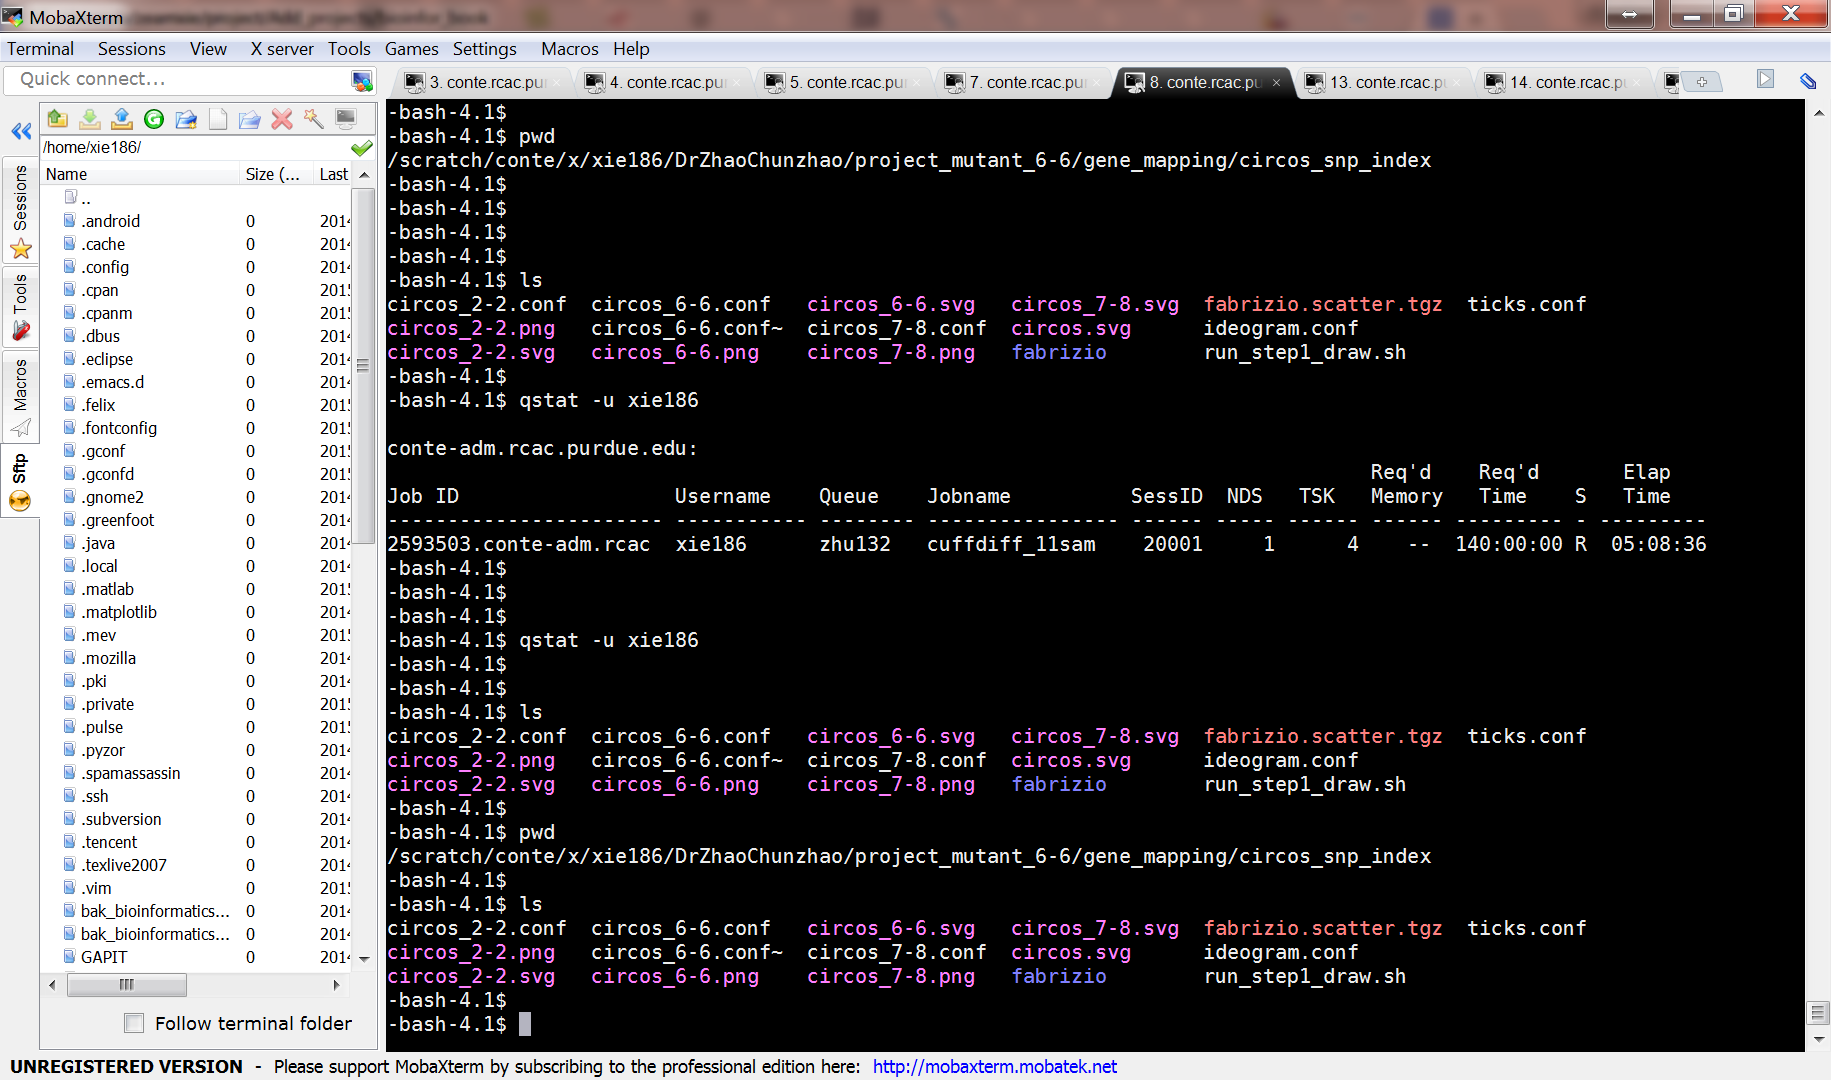
\includegraphics[width=1\linewidth]{figures/linux_terminal_example} 

}

\caption{An example of Linux terminal.}\label{fig:LinuxTerminal}
\end{figure}

Linux is a clone of the operating system Unix, written from scratch by
Linus Torvalds (Figure \ref{fig:LinusTorvaldsGitHub}) with assistance
from a loosely-knit team of hackers across the Net. It aims towards
POSIX and Single UNIX Specification compliance (\citet{Torvalds2015}).

It has all the features you would expect in a modern fully-fledged Unix,
including true multitasking, virtual memory, shared libraries, demand
loading, shared copy-on-write executables, proper memory management, and
multistack networking including IPv4 and IPv6. It is distributed under
the GNU General Public (Torvalds, 2015).

Maybe it's hard to understand what Linux or to remember the sentences
mentioned above. Just know Linux is an operating system like Windows.
This is enough for you to start out.

\begin{figure}

{\centering 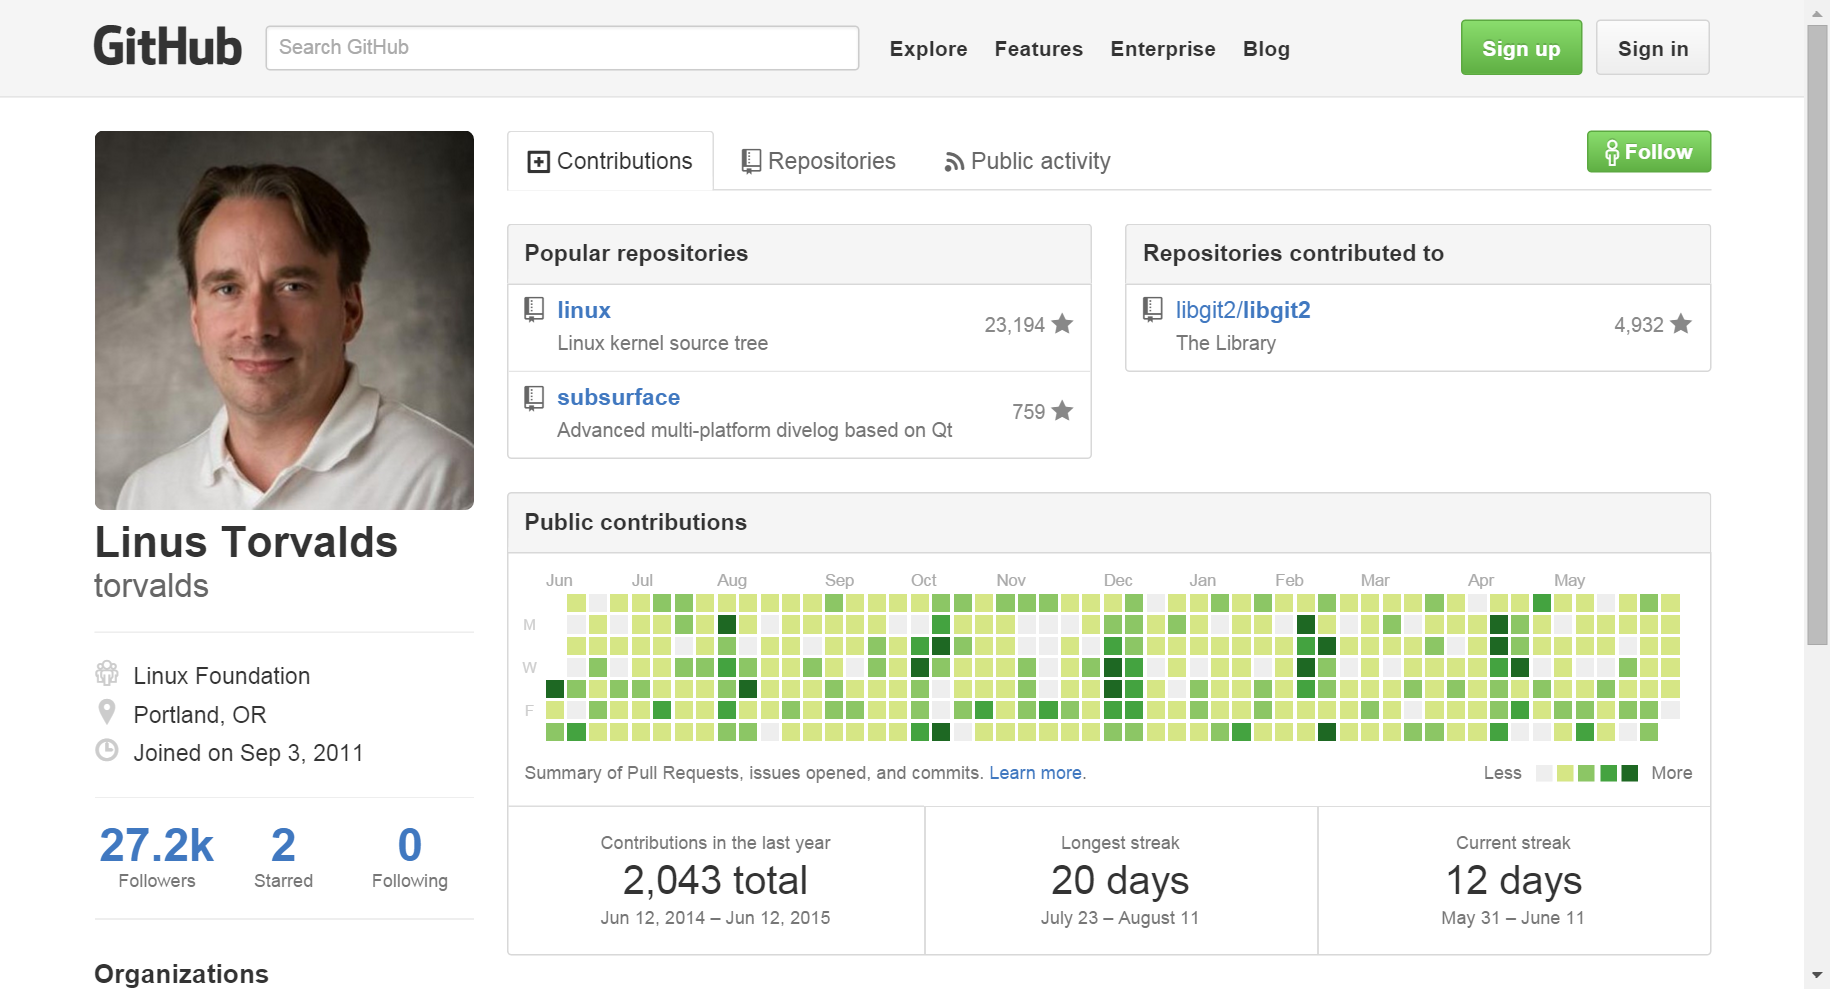
\includegraphics[width=0.5\linewidth]{figures/Linus_Torvalds_GitHub} 

}

\caption{Linus Torvalds on GitHub}\label{fig:LinusTorvaldsGitHub}
\end{figure}

\section{Linux for bioinformatics}\label{linux-for-bioinformatics}

For analysis of NGS data, a large amount of software were developed for
using under Linux environment. Among them, a large proportion can be
only used under Linux environment.

\begin{itemize}
\tightlist
\item
  Easy to build simple pipelines (awk, bash, piping, bash redirection,
  texttools)
\item
  Simple to install and use software development tools
\item
  Multiple versions of a program can be installed by the user himself
  and switched on/off with sourcing some scripts without being
  administrator
\item
  A lot of good scientific software is written in a non portable way for
  linux/unix (almost all short read aligners, samtools). This makes it
  necessary to use Unix for genomics.
\item
  Ability to perform analyses on computer clusters (important for
  big/long computational jobs)
\end{itemize}

\chapter{Connecting to Linux}\label{connecting-to-linux}

\section{User interfaces}\label{user-interfaces}

As an operating systemsm, Linux comes with two types of user interfaces:
Graphical User Interface (GUI) and command line interface (shell).

GUI means there will be window, buttons, menus, etc. The most popular
system with GUI is Windows system (Figure \ref{fig:windowsGUI}).



\begin{figure}
\centering
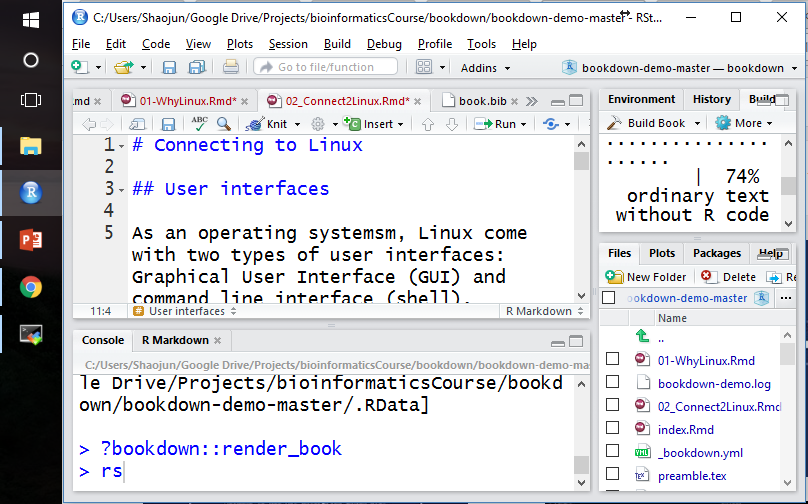
\includegraphics{figures/windows_gui.png}
\caption{\label{fig:windowsGUI}Windows GUI.}
\end{figure}

Command line interfaces means that you need to type the command line
yourself. Usually the results will be displayed as text (Figure
\ref{fig:linuxTerminalExam2}).



\begin{figure}
\centering
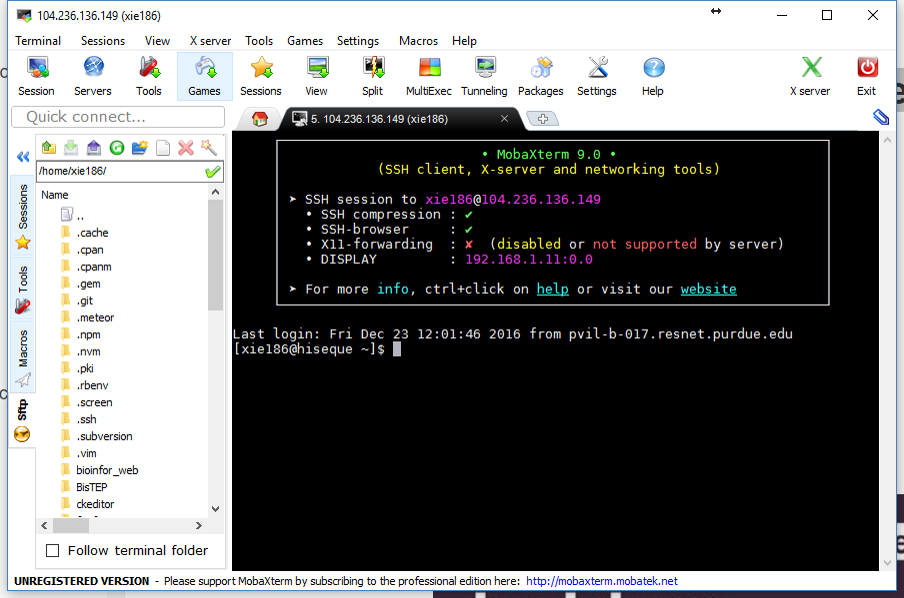
\includegraphics{figures/linux_terminal_exam2.png}
\caption{\label{fig:linuxTerminalExam2}An example of Linux terminal.}
\end{figure}

In Bioinformatics analysis, usually you won't operate directly on the
physical machine of the Linux server. Usually you need to connect to the
Linux server via a tool, like Putty, Mobaxterm, etc.

\section{How to connect}\label{how-to-connect}

If you want to connect to a Linux server, what you need to know first
is:

\begin{enumerate}
\def\labelenumi{\arabic{enumi})}
\item
  IP address of your Linux server;
\item
  User name and password of your account;
\end{enumerate}

If you are a Mac OS X user, you can connect to a Linux server by using
\texttt{Terminal}, a console program included with the operating system.

For Windows users, I would recommend MobaXterm for remote connection.
MobatXterm is an excellent toolbox for remote connection from Windows
system. It comes with an X11 server and provides many networking tools
and tabbed SSH. It has all the essential UNIX commands in a single
portable executable file.

Here I show one example of what you should do When you first open
Mobaxterm. You need to follow the numbers in Figure
\ref{fig:mobaxtermInit}: click \texttt{Session}; then click
\texttt{SSH}; type the IP or name address of the remote host, check
\texttt{Specify\ username} if you need; click \texttt{OK}.



\begin{figure}
\centering
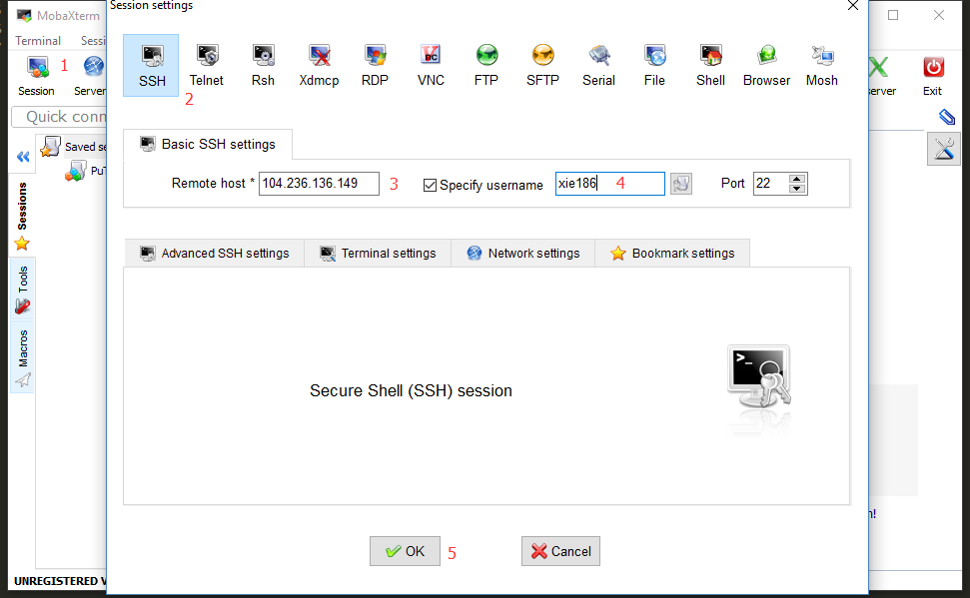
\includegraphics{figures/mobaxterm_init.png}
\caption{\label{fig:mobaxtermInit}First open of Mobaxterm.}
\end{figure}

Then you need to type the password. It's OK that you don't see anything
when you're typing (Figure \ref{fig:mobaxtermSavepswd}). Then click
\texttt{Enter} on the keyboard.For the first time of log-in, you'll be
asked to whether to save the password or not. If you say click
\texttt{Yes}, you won't need to type the password again next time.



\begin{figure}
\centering
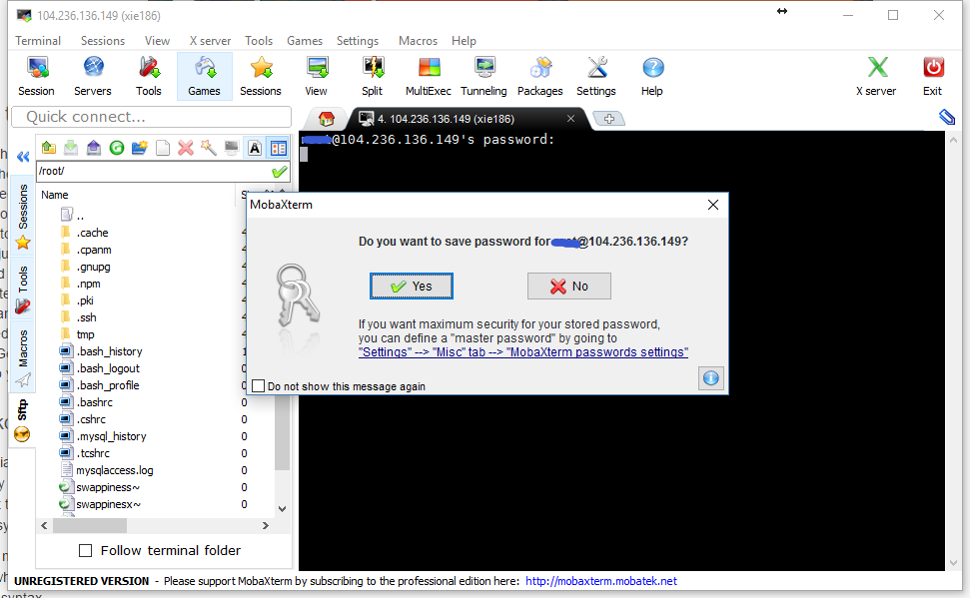
\includegraphics{figures/mobaxterm_savepassword.png}
\caption{\label{fig:mobaxtermSavepswd}Type password and save it in Mobaxterm.}
\end{figure}

If you can find a Linux server, it'll be very good. If NOT, here I
provided a guest account for you. Here are the user name and password:

\begin{verbatim}
IP address: 198.211.107.37
User name: guest4bioinfo
Password: nobigfile
\end{verbatim}

As you can tell from the password, please do NOT upload BIG files
(bigger than 2 MB).

\subsection{Set up Linux Lab
Environment}\label{set-up-linux-lab-environment}

One way to get access to a Linux system is to take advantage of Red Hat
Enterprise Linux delivered by Amazon EC2 (Elastic Compute Cloud). Red
Hat and Amazon Web Services collaborate to provide official Red Hat
Enterprise Linux licensed images through Amazon's on-demand public cloud
service at free or low cost.

The guided exercises and labs for this course were written assuming that
you will set up an account with Amazon Web Services and use it to start
a single, simple system running Red Hat Enterprise Linux 7. You will
connect to that system securely over the internet and use it to practice
commands.

At the time of writing, Amazon Web Services provides an AWS Free Tier
offering, which gives new users free access to certain sizes of cloud
instances and operating environments (including Red Hat Enterprise Linux
7) for up to 750 hours per month, for 12 months.

\BeginKnitrBlock{rmdtip}
\textbf{Install \texttt{samtools} without root previledges}

If you are not eligible for AWS Free Tier or have used up your free tier
eligibility, a t2.micro-sized instance (cloud computer) running the same
software, is currently estimated to cost between US\$0.072 and US\$0.08
per hour of compute time, depending on the data center in which the
instance is started.

To conserve compute time and any costs, make sure you shut down your
cloud instance when you are not using it, and terminate (delete) it when
you are completely finished with it.
\EndKnitrBlock{rmdtip}

\section{Transferring files between local computer and Linux
server}\label{transferring-files-between-local-computer-and-linux-server}

To transfer files between local computer and Linux sever, there are two
options: 1) GUI application and 2) command line.

\begin{itemize}
\tightlist
\item
  Open FileZilla and then click \texttt{File} -\textgreater{}
  \texttt{Site\ Manager}.
\end{itemize}

GUI means there will be window, buttons, menus, etc. The most popular
system with GUI is Windows system (Figure
@ref(fig:filezilla\_screenshot1)).

(ref:filezilla\_screenshot1) FileZilla application.

\begin{figure}
\centering
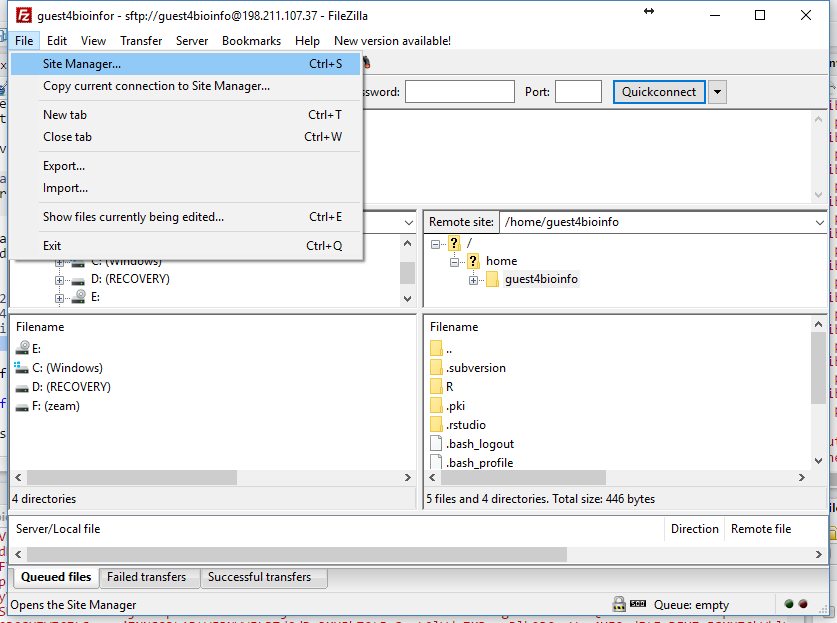
\includegraphics{figures/filezilla_screenshot1.png}
\caption{(\#fig:filezilla\_screenshot1)Windows GUI.}
\end{figure}

\subsection{Use command line tools}\label{use-command-line-tools}

\texttt{rsync} compares the files at each end and transfers only the
changed parts of changed files. When you transfer files the first timeo
it behaves pretty much like scp, but for a second transfer, where most
files are unchanged, it will push a lot less data than scp. It's also a
convenient way to restart failed transfers - you just reissue the same
command and it will pick up where it left off the time before, whereas
scp will start again from scratch.

\subsubsection{\texorpdfstring{Copy files using
\texttt{rsync}}{Copy files using rsync}}\label{copy-files-using-rsync}

\begin{verbatim}
\end{verbatim}

\subsubsection{\texorpdfstring{Copying Files with
\texttt{scp}}{Copying Files with scp}}\label{copying-files-with-scp}

The command \texttt{scp} is short for secure copy. It can be used to
copy files between hosts on a network. It uses ssh(1) for data transfer,
and uses the same authentication and provides the same security as
ssh(1).\texttt{Scp} will ask for passwords or passphrases if they are
needed for authentication.

File names may contain a user and host specification to indicate that
the file is to be copied to/from that host. Local file names can be made
explicit using absolute or relative pathnames to avoid scp treating file
names containing `:' as host specifiers. Copies between two remote hosts
are also permitted.

\begin{Shaded}
\begin{Highlighting}[]
\CommentTok{# Copy the file test.pl on 198.211.107.37 to the current directory.}
\FunctionTok{scp}\NormalTok{ guest4bioinfor@198.211.107.37:~/test.pl ./}
\end{Highlighting}
\end{Shaded}

To copy files from a server to a client, you need to know where the
files are located on the server. For example, to copy a single file
\texttt{\textasciitilde{}/test.pl} from the server with IP address of
198.211.107.37 to the current directory.

\begin{Shaded}
\begin{Highlighting}[]
\CommentTok{# Copy the file test.pl in the current directory to  198.211.107.37}
\FunctionTok{scp}\NormalTok{ ./test.pl guest4bioinfor@198.211.107.37:~/}
\end{Highlighting}
\end{Shaded}

To copy files from a client to a server, you need to know where the
files you want to put on the server. For example, to copy a single file
\texttt{test.pl} from the current folder to the HOME folder of the
server with IP address of 198.211.107.37.

If you want to copy an entire directory recursively, you can use
\texttt{-r} argument. See the example below:

\begin{Shaded}
\begin{Highlighting}[]
\CommentTok{# Copy the file test.pl in the current directory to  198.211.107.37}
\FunctionTok{scp}\NormalTok{ -r guest4bioinfor@198.211.107.37:~/bioinfo/ ./}
\end{Highlighting}
\end{Shaded}

\subsection{Download files}\label{download-files}

\begin{verbatim}
wget <url>
\end{verbatim}

Resume

\begin{verbatim}
wget -c <url>  
\end{verbatim}

Reference:

RH066x Fundamentals of Red Hat Enterprise Linux on edX

\chapter{File system and commands of
Linux}\label{file-system-and-commands-of-linux}

\section{Path}\label{path}

To understand Linux file system, you can image it as a tree structure
(Figure \ref{fig:linuxTreeStruc}).



\begin{figure}
\centering
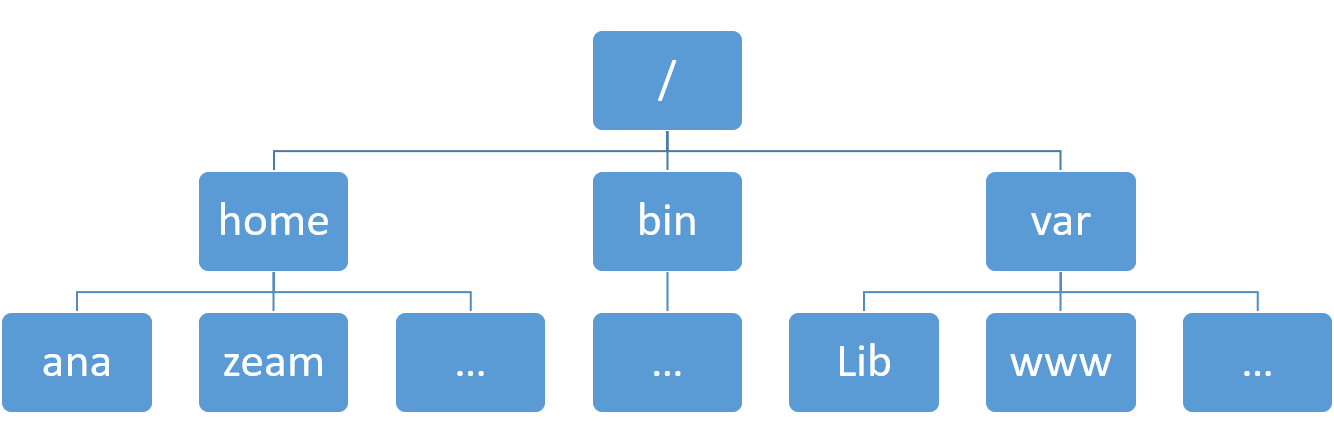
\includegraphics{figures/LinuxPathTree.png}
\caption{\label{fig:linuxTreeStruc}Tree structure of Linux system.}
\end{figure}

In Linux, a path is a unique location of a file or a directory in the
file system.

For convenience, Linux file system is usually thought of in a tree
structure. On a standard Linux system you will find the layout generally
follows the scheme presented below.

The tree of the file system starts at the trunk or slash, indicated by a
forward slash (/). This directory, containing all underlying directories
and files, is also called the root directory or ``the root'' of the file
system.

\subsection{Relative and absolute
path}\label{relative-and-absolute-path}

\begin{itemize}
\tightlist
\item
  \textbf{Absolute path}
\end{itemize}

An absolute path is defined as the location of a file or directory from
the root directory(/). An absolute path starts from the \texttt{root} of
the tree (\texttt{/}).

Here are some examples:

\begin{verbatim}
/home/xie186
/home/xie186/perl5
\end{verbatim}

\begin{itemize}
\tightlist
\item
  \textbf{Relative path}
\end{itemize}

Relative path is a path related to the present working directory.

\begin{verbatim}
data/sample1/
../doc/
\end{verbatim}

If you want to get the \textbf{absolute path} based on \textbf{relative
path}, you can use \texttt{readlink} with parameter \texttt{-f}:

\begin{Shaded}
\begin{Highlighting}[]
\BuiltInTok{pwd}
\FunctionTok{readlink}\NormalTok{ -f ../}
\end{Highlighting}
\end{Shaded}

\begin{verbatim}
## /home/xie186/bookdown/novice2expert4bioinformatics
## /home/xie186/bookdown
\end{verbatim}

\section{Surfing in Linux file
system}\label{surfing-in-linux-file-system}

Once we enter into a Linux file system, we need to 1) know where we are;
2) how to get where we want; 3) how to know what files or directories we
have in a particular path.

\subsection{\texorpdfstring{Command
\texttt{pwd}}{Command pwd}}\label{command-pwd}

In order to know where we are, we need to use \texttt{pwd} command. The
command \texttt{pwd} is short for ``print name of current/working
directory''. It will return the full path of current directory.

Command pwd is almost always used by itself. This means you only need to
type pwd and press ENTER (Figure \ref{fig:linuxCMDpwd}).



\begin{figure}

{\centering 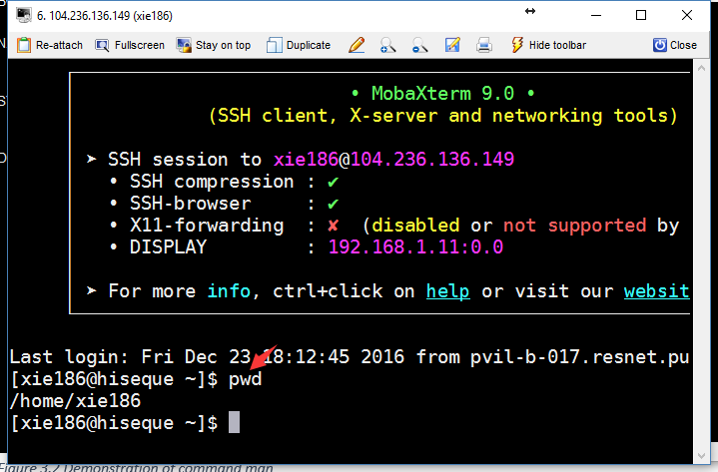
\includegraphics[width=0.8\linewidth]{figures/linuxCMDpwd} 

}

\caption{ref:linuxCMDpwd}\label{fig:linuxCMDpwd}
\end{figure}

\subsection{\texorpdfstring{Comand
\texttt{ls}}{Comand ls}}\label{comand-ls}

After you know where you are, then you want to know what you have in
that directory, we can use command \texttt{ls} to list directory
contents (Figure \ref{fig:linuxCMDls}). Its syntax is:

\begin{verbatim}
ls [option]... [file]...
\end{verbatim}



\begin{figure}

{\centering 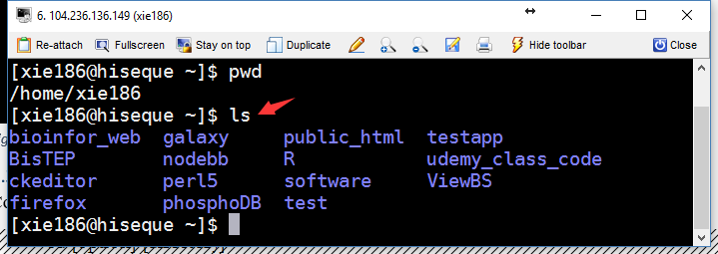
\includegraphics[width=0.8\linewidth]{figures/linuxCMDls} 

}

\caption{ref:linuxCMDls}\label{fig:linuxCMDls}
\end{figure}

\texttt{ls} with no option will list files and directories in bare
format. Bare format means the detailed information (type, size, modified
date and time, permissions and links etc) won't be viewed. When you use
\texttt{ls} by itself (Figure \ref{fig:linuxCMDls}), it will list files
and directories in the current directory.

\subsection{\texorpdfstring{Command
\texttt{cd}}{Command cd}}\label{command-cd}

Command cd is used to change the current directory. It's syntax is:

\begin{verbatim}
cd [option] [directory]
\end{verbatim}

Unlike \texttt{pwd}, when you use \texttt{cd} you usually need to
provide the path (either absolute or relative path) which we want to
enter.

If we didn't provide any path information, we will change to home
directory by default.

\section{Path shortcuts}\label{path-shortcuts}

In Linux, there are three commonly used path shortpaths (Table
\ref{tab:linuxPathShortcuts}).



\begin{table}

\caption{\label{tab:linuxPathShortcuts}Shortcuts of path.}
\centering
\begin{tabular}[t]{c|c|c}
\hline
Path & Shortcuts & Description\\
\hline
Single dot & . & The current folder\\
\hline
Double dots & .. & The folder above the current folder\\
\hline
Tilde character & \textasciitilde{} & Home directory (normally the directory:/home/my\_login\_name)\\
\hline
\end{tabular}
\end{table}

Here are some examples:

\begin{Shaded}
\begin{Highlighting}[]
\CommentTok{### }
\BuiltInTok{cd}\NormalTok{ ~}
\BuiltInTok{pwd}
\FunctionTok{ls}
\end{Highlighting}
\end{Shaded}

\begin{verbatim}
/home/xie186
bak
bin
bookdown
cpanm
curl-7.55.0
curl-7.55.0.tar.gz
github_repo
meteor
meteor-window-manager
perl5
R
software
ViewBS
\end{verbatim}

\begin{Shaded}
\begin{Highlighting}[]

\CommentTok{##}

\FunctionTok{ls}\NormalTok{ ./}
\end{Highlighting}
\end{Shaded}

\begin{verbatim}
01-WhyLinux.Rmd
02_Connect2Linux.Rmd
03_FileSystemLinux.Rmd
04_Linux_FilteringOutputandFindingThings.Rmd
05-TextEditorInLinux.Rmd
06_InstallationOfSoftwareInLinux.Rmd
07_AchivingAndCompressingFiles.Rmd
07-FirstPerlProgram.Rmd
07-PerlArrat.Rmd
08-PerlVariableOperator.Rmd
09_PerlControlStructure.Rmd
09_StringManipulationRegExp.Rmd
10_PerlInputOutput.Rmd
10_PerlModules.Rmd
10_Rbasics.Rmd
10_SimpleGraphR.Rmd
112_GenerateHeatmap.Rmd
11_FigureManuscript.Rmd
11_GenomeSequence.Rmd
11_IntronNGS.Rmd
11_practicalPerlProgram.Rmd
11_StringManipulationRegExp.Rmd
12_RNA-seq.Rmd
13_BSseq.Rmd
14_WhatLinuxShellIS.Rmd
18_CapstoneProject.Rmd
18_Good_resource.Rmd
19_Python.Rmd
20_R_intro.Rmd
21_Reference.Rmd
bioinfBookXIE186.aux
bioinfBookXIE186_files
bioinfBookXIE186.log
bioinfBookXIE186.Rmd
_book
book.bib
bookdown-demo_files
bookdown-demo.log
bookdown-demo.Rproj
_bookdown_files
_bookdown.yml
_build.sh
code_perl
code_python
code_R
data
_deploy.sh
DESCRIPTION
figures
images
index.Rmd
LICENSE
_output.yml
packages.bib
preamble_bak.tex
preamble.tex
README.md
rpres.css
style.css
tables
toc.css
\end{verbatim}

\begin{Shaded}
\begin{Highlighting}[]

\CommentTok{## }
\BuiltInTok{pwd}
\BuiltInTok{cd}\NormalTok{ ../}
\BuiltInTok{pwd}
\BuiltInTok{cd}\NormalTok{ ./}
\BuiltInTok{pwd}
\end{Highlighting}
\end{Shaded}

\begin{verbatim}
/home/xie186/bookdown/novice2expert4bioinformatics
/home/xie186/bookdown
/home/xie186/bookdown
\end{verbatim}

Each directory has two entries in it at the start, with names . (a link
to itself) and .. (a link to its parent directory). The exception, of
course, is the root directory, where the .. directory also refers to the
root directory.

\section{Manipulations of files and
directories}\label{manipulations-of-files-and-directories}

In Linux, manipulations of files and directories are the most frequent
work. In this section, you will learn how to copy, rename, remove, and
create files and directories.

\subsection{\texorpdfstring{Command
\texttt{cp}}{Command cp}}\label{command-cp}

In Linux, command \texttt{cp} can help you copy files and directories
into a target directory.

\subsection{\texorpdfstring{Command
\texttt{mv}}{Command mv}}\label{command-mv}

The command \texttt{mv} is short for move (or rename) files.

\subsubsection{Move one file}\label{move-one-file}

Here is one common example of \texttt{mv}.

\begin{Shaded}
\begin{Highlighting}[]

\FunctionTok{mv}\NormalTok{ file1 directory1/}
\end{Highlighting}
\end{Shaded}

\subsubsection{Move multiple files into a
directory}\label{move-multiple-files-into-a-directory}

\begin{Shaded}
\begin{Highlighting}[]
\FunctionTok{mv}\NormalTok{ file1 file2 file3 target_direcotry/}
\end{Highlighting}
\end{Shaded}

\subsubsection{Move a directory}\label{move-a-directory}

\begin{Shaded}
\begin{Highlighting}[]
\FunctionTok{mv}\NormalTok{ dir1}
\end{Highlighting}
\end{Shaded}

\subsubsection{Rename a file or a
directory}\label{rename-a-file-or-a-directory}

\subsection{\texorpdfstring{Command
\texttt{mkdir}}{Command mkdir}}\label{command-mkdir}

Command \texttt{mkdir} is short for make directory.

The syntax is shown as below:

\begin{verbatim}
mkdir [OPTION ...] DIRECTORY ...
\end{verbatim}

\begin{Shaded}
\begin{Highlighting}[]
\FunctionTok{mkdir}\NormalTok{ directory}
\end{Highlighting}
\end{Shaded}

Multiple directories can be specified when calling \texttt{mkdir}.

\begin{Shaded}
\begin{Highlighting}[]
\FunctionTok{mkdir}\NormalTok{ directory1 directory2}
\end{Highlighting}
\end{Shaded}

\subsubsection{How to create a}\label{how-to-create-a}

\begin{verbatim}
mkdir -p foo/bar/baz
\end{verbatim}

\begin{quote}
How to defining complex directory trees with one command
\end{quote}

\begin{verbatim}
mkdir -p project/{software,results,doc/{html,info,pdf},scripts}
\end{verbatim}

This will create a direcotry trees as shown below:

\begin{verbatim}
$ tree project/
project/
├── doc
│   ├── html
│   ├── info
│   └── pdf
├── results
├── scripts
└── software

7 directories, 0 files
\end{verbatim}

The command line above will directories \texttt{foo}, \texttt{foo/bar},
and \texttt{foo/bar/baz} if they don't exist.

\section{Viewing text files in Linux}\label{viewing-text-files-in-linux}

\subsection{\texorpdfstring{Command
\texttt{cat}}{Command cat}}\label{command-cat}

The command \texttt{cat} is short for concatenate files and print on the
standard output.

The syntax is shown as below:

\begin{verbatim}
cat [OPTION]... [FILE]...
\end{verbatim}

For small text file, \texttt{cat} can be used to view the files on the
standard output.

\begin{Shaded}
\begin{Highlighting}[]
\FunctionTok{cat}\NormalTok{ data/testdata4linux_cmd.txt}
\end{Highlighting}
\end{Shaded}

\begin{verbatim}
## gene1
## gene2
## gene3
## gene4
## gene5
## gene6
## gene7
## gene8
## gene9
## gene10
## gene11
## gene12
## gene13
## gene14
## gene15
## gene16
\end{verbatim}

You can also use \texttt{cat} to merge two text files.

\begin{Shaded}
\begin{Highlighting}[]
\FunctionTok{cat}\NormalTok{ file1 file2 }\OperatorTok{>}\NormalTok{ merged_file}
\end{Highlighting}
\end{Shaded}

\subsection{\texorpdfstring{Command \texttt{more} and
\texttt{less}}{Command more and less}}\label{command-more-and-less}

The command \texttt{more} is old utility. When the text passed to it is
too large to fit on one screen, it pages it. You can scroll down but not
up.

The syntaxt of \texttt{more} is shown below:

\begin{verbatim}
more [options] file [...]
\end{verbatim}

The command \texttt{less} was written by a man who was fed up with
more's inability to scroll backwards through a file. He turned less into
an open source project and over time, various individuals added new
features to it. less is massive now. That's why some small embedded
systems have more but not less. For comparison, less's source is over
27000 lines long. more implementations are generally only a little over
2000 lines long.

The syntaxt of \texttt{less} is shown below:

\begin{verbatim}
less [options] file [...]
\end{verbatim}

\subsection{\texorpdfstring{Command \texttt{head} and
\texttt{tail}}{Command head and tail}}\label{command-head-and-tail}

The command \texttt{head} is used to output the first part of files. By
default, it outputs the first 10 lines of the file.

\begin{verbatim}
head [OPTION]... [FILE]...
\end{verbatim}

Here is an exmaple of printing the first 5 files of the file:

\begin{Shaded}
\begin{Highlighting}[]
\FunctionTok{head}\NormalTok{ -n 5 code_perl/variable_assign.pl}
\end{Highlighting}
\end{Shaded}

\begin{verbatim}
## #!/usr/bin/perl
## use warnings;
## use strict;
## 
## #assign two strings to two variables
\end{verbatim}

In fact, the letter n does not even need to be used at all. Just the
hyphen and the integer (with no intervening space) are sufficient to
tell head how many lines to return. Thus, the following would produce
the same result as the above commands:

\begin{Shaded}
\begin{Highlighting}[]
\FunctionTok{head}\NormalTok{ -5 data/testdata4linux_cmd.txt}
\end{Highlighting}
\end{Shaded}

\begin{verbatim}
## gene1
## gene2
## gene3
## gene4
## gene5
\end{verbatim}

The command \texttt{tail} is used to output the last part of files. By
default, it prints the last 10 lines of the file to standard output.

The syntax is shown below:

\begin{verbatim}
tail [OPTION]... [FILE]...
\end{verbatim}

Here is an exmaple of printing the last 5 files of the file:

\begin{Shaded}
\begin{Highlighting}[]
\FunctionTok{tail}\NormalTok{ -5 data/testdata4linux_cmd.txt}
\end{Highlighting}
\end{Shaded}

\begin{verbatim}
## gene12
## gene13
## gene14
## gene15
## gene16
\end{verbatim}

To view lines from a specific point in a file, you can use
\texttt{-n\ +NUMBER} with the \texttt{tail} command. For example, here
is an example of viewing the file from the 2nd line of the line.

\begin{Shaded}
\begin{Highlighting}[]
\FunctionTok{tail}\NormalTok{ -n +2 data/testdata4linux_cmd.txt}
\end{Highlighting}
\end{Shaded}

\begin{verbatim}
## gene2
## gene3
## gene4
## gene5
## gene6
## gene7
## gene8
## gene9
## gene10
## gene11
## gene12
## gene13
## gene14
## gene15
## gene16
\end{verbatim}

\subsection{Auto-completion}\label{auto-completion}

In most Shell environment, programmable completion feature will also
improve your speed of typing. It permits typing a partial name of
command or a partial file (or directory), then pressing \texttt{TAB} key
to auto-complete the command (Figure \ref{fig:linuxAutoCompletion}). If
there are more than one possible completions, then TAB will list all of
them (Figure \ref{fig:linuxAutoCompletion}).




\begin{figure}
\centering
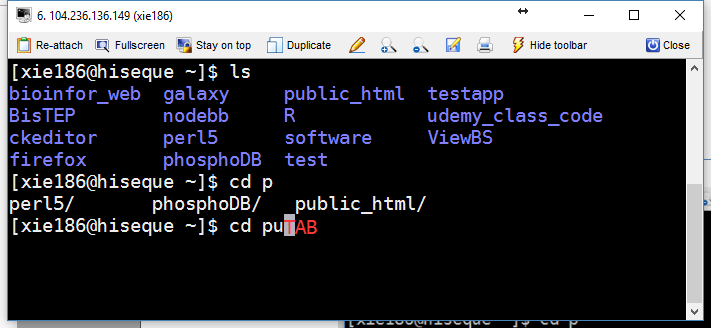
\includegraphics{figures/linuxAutoCompletion.png}
\caption{\label{fig:linuxAutoCompletion}Demonstration of programmable completion
feature.}
\end{figure}

\section{Understand standard input and stardard
output}\label{understand-standard-input-and-stardard-output}

In the Linux environment, input and output is distributed across three
streams: standard input (STDIN), standard output (STDOUT), standard
error (STDERR). These three streams are also numbered: STDIN (0), STDOUT
(1), STDERR (2).

\subsection{STDIN}\label{stdin}

\ldots{} The standard input stream typically carries data from a user to
a program. Programs that expect standard input usually receive input
from a device, such as a keyboard. Standard input is terminated by
reaching EOF (end-of-file). As described by its name, EOF indicates that
there is no more data to be read.

To see standard input in action, run the cat program. Cat stands for
concatenate, which means to link or combine something. It is commonly
used to combine the contents of two files. When run on its own, cat
opens a looping prompt. \ldots{}

\begin{verbatim}
tail
1
2
3
`CTRL+D`
1
2
3
\end{verbatim}

\subsection{STDOUT}\label{stdout}

Data that is generated by a program will be written by STDOUT. If the
STDOUT is not redirected, it will output the data on to the terminal.

\begin{Shaded}
\begin{Highlighting}[]
\VariableTok{stdout=}\StringTok{"Hello world"}
\BuiltInTok{echo} \VariableTok{$stdout}
\end{Highlighting}
\end{Shaded}

\begin{verbatim}
## Hello world
\end{verbatim}

The STDOUT can be redirected to a file. See the example below:

\begin{Shaded}
\begin{Highlighting}[]
\VariableTok{stdout=}\StringTok{"Hello world"}
\BuiltInTok{echo} \VariableTok{$stdout} \OperatorTok{>}\NormalTok{ data/test_output.txt}
\CommentTok{# cat the data}
\FunctionTok{cat}\NormalTok{ data/test_output.txt}
\end{Highlighting}
\end{Shaded}

\begin{verbatim}
## Hello world
\end{verbatim}

\subsection{STDERR}\label{stderr}

During a program's execution, some errors may be generated when the
program fails at some parts. STDERR will help you write the errors. By
default, the STDERR will be outputed onto the terminal.

Here is an example of STDERR

\begin{Shaded}
\begin{Highlighting}[]
\FunctionTok{ls}\NormalTok{ NOTAFILE}
\end{Highlighting}
\end{Shaded}

\begin{verbatim}
## ls: cannot access NOTAFILE: No such file or directory
\end{verbatim}

\section{Auto-completion}\label{auto-completion-1}

A handy autocomplete feature also exists. Type one or more letters,
press the Tab key twice, and then a list of functions starting with
these letters appears. For example: type so, press the Tab key twice,
and then you get the list as: sort sort! sortby sortby! sortcols
sortperm sortrows.

\section{}\label{section}

Filtering Output and Finding Things

\url{https://www.youtube.com/playlist?list=PLtK75qxsQaMLZSo7KL-PmiRarU7hrpnwK}

\section{Check you job status}\label{check-you-job-status}

\begin{verbatim}
$ ps aux  
USER       PID  %CPU %MEM  VSZ RSS     TTY   STAT START   TIME COMMAND
timothy  29217  0.0  0.0 11916 4560 pts/21   S+   08:15   0:00 pine  
root     29505  0.0  0.0 38196 2728 ?        Ss   Mar07   0:00 sshd: can [priv]   
can      29529  0.0  0.0 38332 1904 ?        S    Mar07   0:00 sshd: can@notty  
\end{verbatim}

USER = user owning the process PID = process ID of the process \%CPU =
It is the CPU time used divided by the time the process has been
running. \%MEM = ratio of the process's resident set size to the
physical memory on the machine VSZ = virtual memory usage of entire
process (in KiB) RSS = resident set size, the non-swapped physical
memory that a task has used (in KiB) TTY = controlling tty (terminal)
STAT = multi-character process state START = starting time or date of
the process TIME = cumulative CPU time COMMAND = command with all its
arguments

\subsection{List files bigger than filesize
specified}\label{list-files-bigger-than-filesize-specified}

\begin{verbatim}
# To find files larger than 100MB:
find . -type f -size +100M
# If you want the current dir only:
find . -maxdepth 1 -type f -size +100M
\end{verbatim}

References:

\url{https://superuser.com/questions/117913/ps-aux-output-meaning}

\chapter{Text editor in Linux}\label{text-editor-in-linux}

In Linux, we sometimes need to create or edit a text file like writing a
new R program. So we need to use text editor.

As a newbie, someone would prefer a basic, GUI-based text editor with
menus and traditional CUA key bindings. Here we recommend
\href{https://www.sublimetext.com/}{Sublime} and
\href{https://notepad-plus-plus.org/}{Notepad++}.

But GUI-based text editor is not always available in Linux. A powerful
screen text editor vi (pronounced ``vee-eye'') is available on nearly
all Linux system. We highly recommend vi as a text editor, because
something we'll have to edit a text file on a system without a
friendlier text editor. Once we get familiar with vi, we'll find that
it's very fast and powerful.

But remember, it's OK if you think this part is too difficult at the
beginning. You can use either Sublime or Notepad++. If you are
connecting to a Linux system without Sublime and Notepad++, you can
write the file in a local computer and then upload the file onto Linux
system (See ).

\section{Basic vi skills}\label{basic-vi-skills}

As vi uses a lot of combination of keystrokes, it may be not easy for
newbies to remember all the combinations in one fell swoop. Considering
this, we'll first introduce the basic skills someone needs to know to
use vi. We need to first understand how three modes of vi work and then
try to remember a few basic vi commonds. Then we can use these skills to
write Perl or R scripts in the following chaptors for Perl and R (Figure
\ref{fig:workingModeVi}).



\begin{figure}
\centering
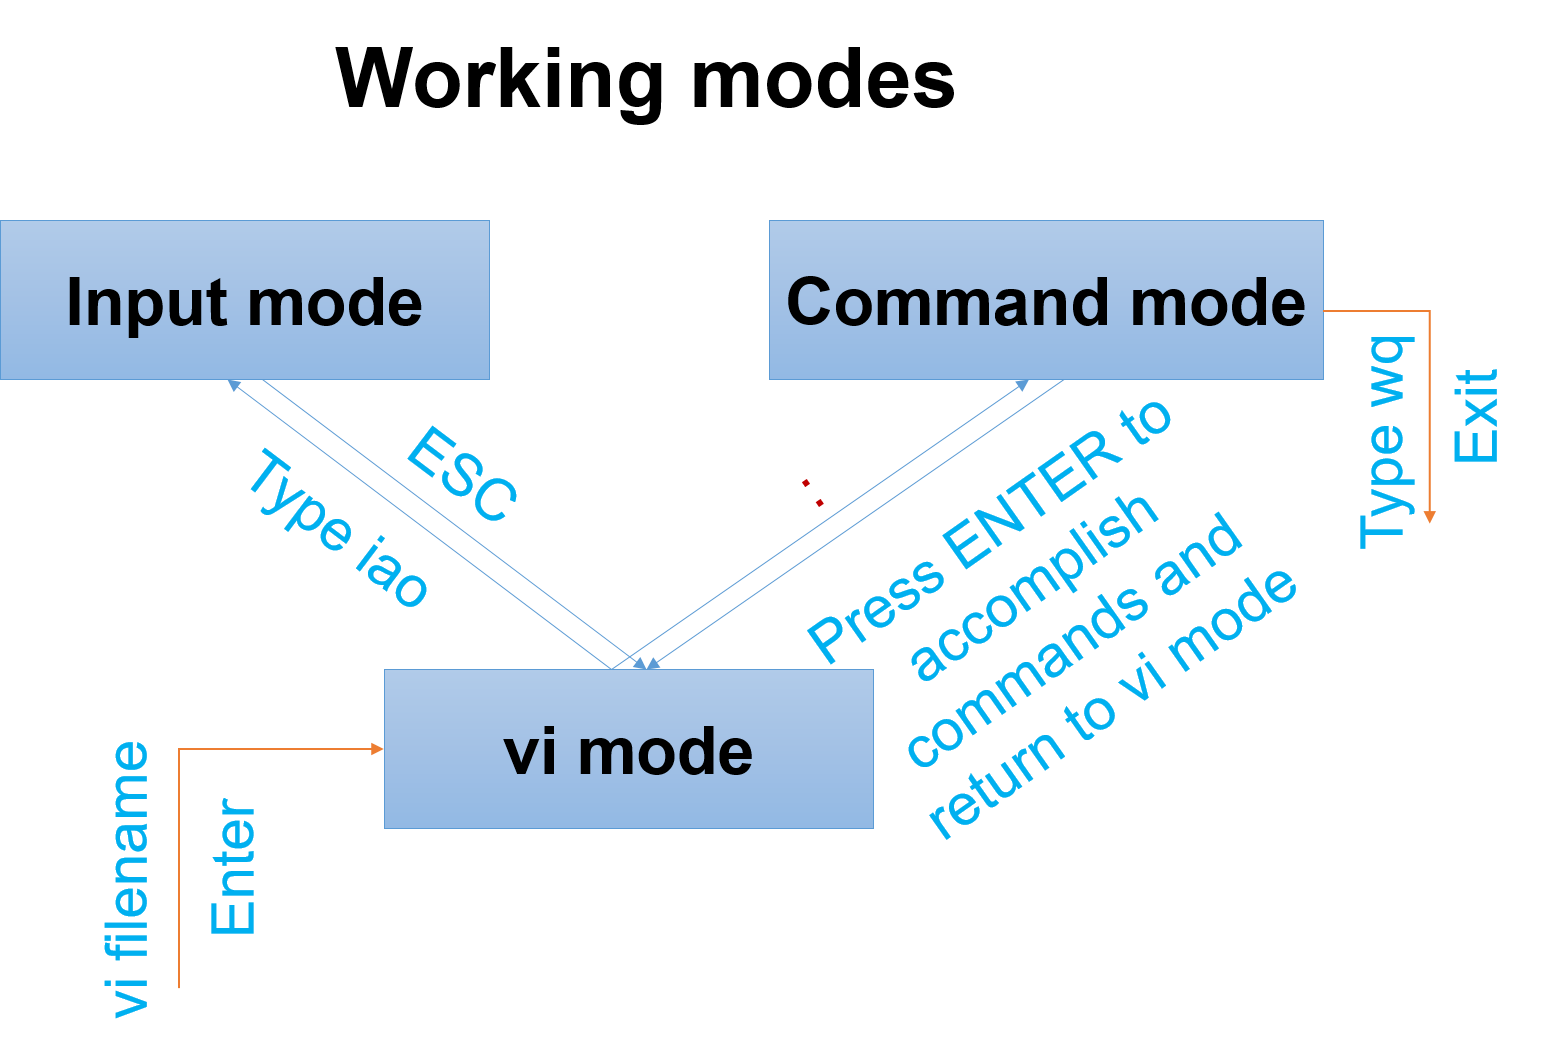
\includegraphics{figures/workingModeVi.png}
\caption{\label{fig:workingModeVi}Three modes of vi.}
\end{figure}

\section{An example for using editor
R}\label{an-example-for-using-editor-r}

\begin{Shaded}
\begin{Highlighting}[]
\KeywordTok{qnorm}\NormalTok{(.}\DecValTok{975}\NormalTok{)}
\end{Highlighting}
\end{Shaded}

\begin{verbatim}
## [1] 1.959964
\end{verbatim}

\begin{Shaded}
\begin{Highlighting}[]
\NormalTok{xval<-}\KeywordTok{seq}\NormalTok{(}\OperatorTok{-}\FloatTok{3.2}\NormalTok{,}\FloatTok{3.2}\NormalTok{, }\DataTypeTok{length=}\DecValTok{1000}\NormalTok{)}
\NormalTok{yval<-}\KeywordTok{dnorm}\NormalTok{(xval)}
\KeywordTok{plot}\NormalTok{(xval, yval, }\DataTypeTok{type=}\StringTok{"l"}\NormalTok{,}\DataTypeTok{axes=}\NormalTok{T,}\DataTypeTok{lwd=}\DecValTok{3}\NormalTok{,}\DataTypeTok{xlab=}\StringTok{""}\NormalTok{,}\DataTypeTok{ylab=}\StringTok{""}\NormalTok{)}
\NormalTok{x<-}\KeywordTok{seq}\NormalTok{(}\KeywordTok{qnorm}\NormalTok{(.}\DecValTok{975}\NormalTok{), }\FloatTok{3.2}\NormalTok{, }\DataTypeTok{length =} \DecValTok{100}\NormalTok{)}
\KeywordTok{polygon}\NormalTok{(}\KeywordTok{c}\NormalTok{(x,}\KeywordTok{rev}\NormalTok{(x)), }\KeywordTok{c}\NormalTok{(}\KeywordTok{dnorm}\NormalTok{(x), }\KeywordTok{rep}\NormalTok{(}\DecValTok{0}\NormalTok{,}\KeywordTok{length}\NormalTok{(x))), }\DataTypeTok{col=}\StringTok{"salmon"}\NormalTok{)}
\KeywordTok{text}\NormalTok{(}\KeywordTok{mean}\NormalTok{(x),}\KeywordTok{mean}\NormalTok{(}\KeywordTok{dnorm}\NormalTok{(x))}\OperatorTok{+}\FloatTok{0.02}\NormalTok{, }\StringTok{"2.5%"}\NormalTok{, }\DataTypeTok{cex=}\DecValTok{2}\NormalTok{)}
\KeywordTok{text}\NormalTok{(}\KeywordTok{qnorm}\NormalTok{(.}\DecValTok{95}\NormalTok{), }\FloatTok{0.01}\NormalTok{, }\StringTok{"1.645"}\NormalTok{,}\DataTypeTok{cex=}\DecValTok{2}\NormalTok{)}

\NormalTok{x<-}\KeywordTok{seq}\NormalTok{(}\OperatorTok{-}\FloatTok{3.2}\NormalTok{, }\KeywordTok{qnorm}\NormalTok{(.}\DecValTok{025}\NormalTok{), }\DataTypeTok{length =}\DecValTok{100}\NormalTok{)}
\KeywordTok{polygon}\NormalTok{(}\KeywordTok{c}\NormalTok{(x,}\KeywordTok{rev}\NormalTok{(x)), }\KeywordTok{c}\NormalTok{(}\KeywordTok{dnorm}\NormalTok{(x), }\KeywordTok{rep}\NormalTok{(}\DecValTok{0}\NormalTok{,}\KeywordTok{length}\NormalTok{(x))), }\DataTypeTok{col=}\StringTok{"salmon"}\NormalTok{)}
\KeywordTok{text}\NormalTok{(}\KeywordTok{mean}\NormalTok{(x),}\KeywordTok{mean}\NormalTok{(}\KeywordTok{dnorm}\NormalTok{(x))}\OperatorTok{+}\FloatTok{0.02}\NormalTok{, }\StringTok{"2.5%"}\NormalTok{, }\DataTypeTok{cex=}\DecValTok{2}\NormalTok{)}
\KeywordTok{text}\NormalTok{(}\KeywordTok{qnorm}\NormalTok{(.}\DecValTok{025}\NormalTok{), }\FloatTok{0.01}\NormalTok{, }\StringTok{"1.645"}\NormalTok{,}\DataTypeTok{cex=}\DecValTok{2}\NormalTok{)}
\end{Highlighting}
\end{Shaded}

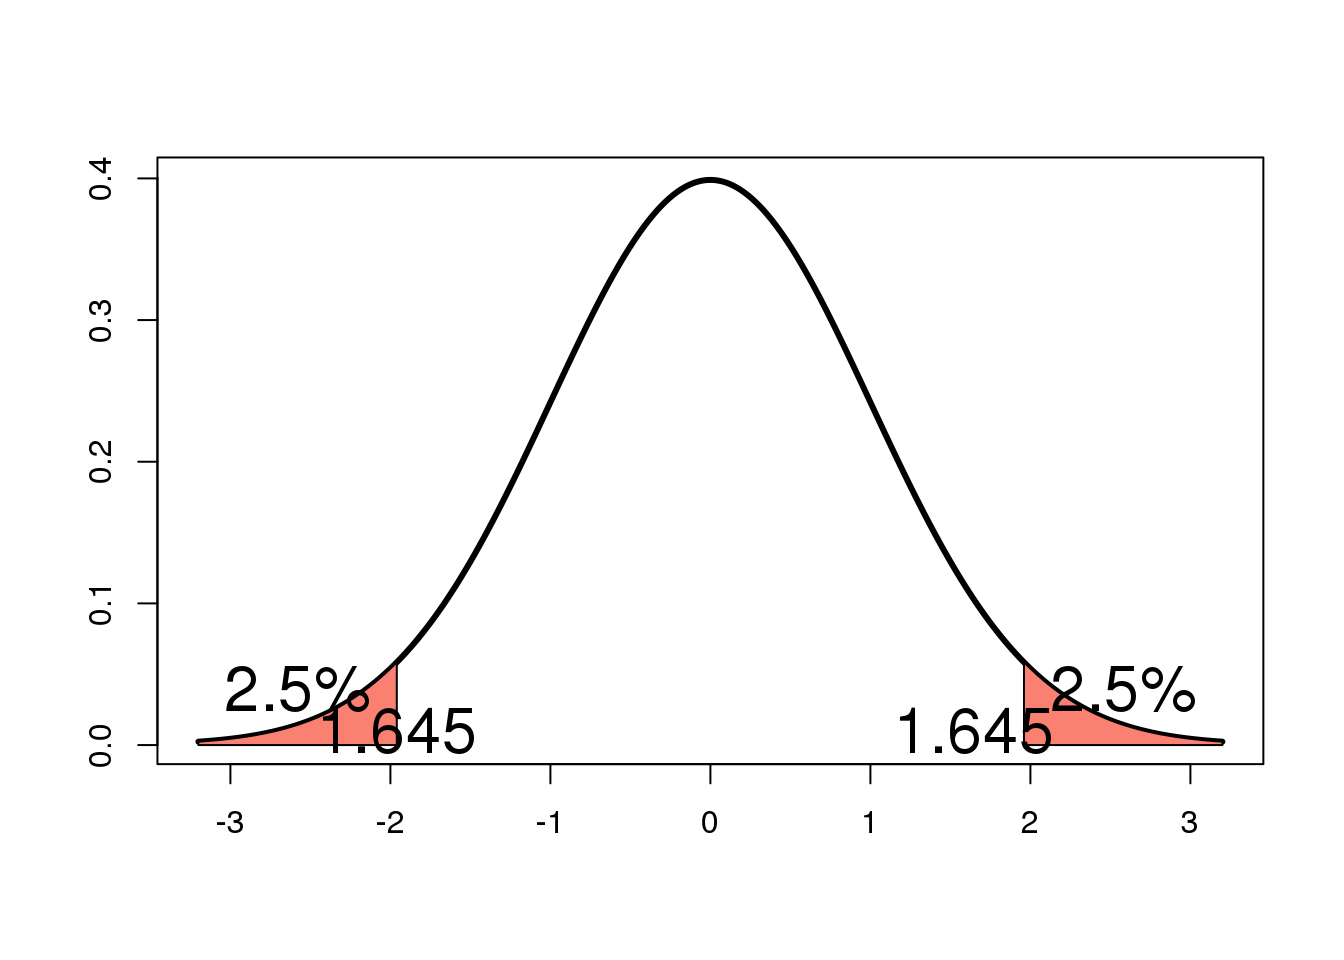
\includegraphics{bioinfBookXIE186_files/figure-latex/unnamed-chunk-24-1.pdf}

\subsection{Shell scipt}\label{shell-scipt}

\url{https://wikis.utexas.edu/display/bioiteam/Example+BWA+alignment+script}

\section{How to exit VIM}\label{how-to-exit-vim}

\url{https://stackoverflow.com/questions/11828270/how-to-exit-the-vim-editor}

\#\# split Vim window to view multiple files at once?

\#\#\#

```

```

\#\#\#

\url{https://stackoverflow.com/questions/1269603/to-switch-from-vertical-split-to-horizontal-split-fast-in-vim}

\url{https://vi.stackexchange.com/questions/64/is-it-possible-to-split-vim-window-to-view-multiple-files-at-once}

\url{https://askubuntu.com/questions/418396/what-is-the-difference-between-vi-and-vim}

\url{https://unix.stackexchange.com/questions/93144/exit-vim-more-quickly}

\url{https://stackoverflow.com/questions/53664/how-to-effectively-work-with-multiple-files-in-vim?rq=1}

\chapter{Install Bioinformatics software in
Linux}\label{install-bioinformatics-software-in-linux}

\section{Installation from source
code}\label{installation-from-source-code}

Nearly all of the Bioinformatics softwares will be downloaded as a
compressed files. So the first thing you need to do is to uncompress the
file. Then the source codes will be included in a folder. You can
\texttt{cd} to the folder and \texttt{ls} the files/directories. Mostly
you will find either a file named \texttt{README} or \texttt{INSTALL} or
both. If you read this file to know how to install the software.

\subsection{\texorpdfstring{Install
\texttt{bwa}}{Install bwa}}\label{install-bwa}

\begin{Shaded}
\begin{Highlighting}[]
\FunctionTok{wget}\NormalTok{ https://sourceforge.net/projects/bio-bwa/files/bwa-0.7.15.tar.bz2}
\FunctionTok{tar}\NormalTok{ xjvf bwa-0.7.15.tar.bz2}
\BuiltInTok{cd}\NormalTok{ bwa-0.7.15}
\FunctionTok{make}
\end{Highlighting}
\end{Shaded}

\subsection{\texorpdfstring{Install
\texttt{samtools}}{Install samtools}}\label{install-samtools}

Installation of \texttt{Samtools} is one of the best representatives of
how to instsall a Bioinformatics tool.

\begin{Shaded}
\begin{Highlighting}[]
\CommentTok{# Download the source code}
\FunctionTok{wget}\NormalTok{ https://iweb.dl.sourceforge.net/project/samtools/samtools/1.3.1/samtools-1.3.1.tar.bz2}
\CommentTok{# Uncompress the source code}
\FunctionTok{tar}\NormalTok{ xjvf samtools-1.3.1.tar.bz2}
\CommentTok{# Enter the source code directory.}
\BuiltInTok{cd}\NormalTok{ samtools-1.3.1}
\CommentTok{# Configure the build system}
\ExtensionTok{./configure}
\CommentTok{# Build samtools}
\FunctionTok{make}
\CommentTok{# Become a `root` user for system-wide install:}
\FunctionTok{su}\NormalTok{ root}
\CommentTok{# Install `Samtools`}
\FunctionTok{make}\NormalTok{ install}
\end{Highlighting}
\end{Shaded}

\BeginKnitrBlock{rmdtip}
\textbf{Install \texttt{samtools} without root previledges}

By default, `make install' installs samtools and the utilities under
/usr/local/bin and manual pages under /usr/local/share/man.

You can specify a different location to install Samtools by configuring
with --prefix=DIR or specify locations for particular parts of HTSlib by
configuring with --bindir=DIR and so on. Type `./configure --help' for
the full list of such install directory options.

Alternatively you can specify different locations at install time by
typing `make prefix=DIR install' or `make bindir=DIR install' and so on.
Consult the list of prefix/exec\_prefix/etc variables near the top of
the Makefile for the full list of such variables that can be overridden.

You can also specify a staging area by typing `make DESTDIR=DIR
install', possibly in conjunction with other --prefix or prefix=DIR
settings. For example,

\begin{verbatim}
make DESTDIR=/tmp/staging prefix=/opt
\end{verbatim}

would install into bin and share/man subdirectories under
/tmp/staging/opt.
\EndKnitrBlock{rmdtip}

\subsection{\texorpdfstring{Align reads to genome using \texttt{bwa} and
store the alignment results in SAM/BAM
files}{Align reads to genome using bwa and store the alignment results in SAM/BAM files}}\label{align-reads-to-genome-using-bwa-and-store-the-alignment-results-in-sambam-files}

\begin{verbatim}
./bwa index ref.fa
./bwa mem ref.fa read-se.fq.gz | gzip -3 > aln-se.sam.gz
./bwa mem ref.fa read1.fq read2.fq | gzip -3 > aln-pe.sam.gz
\end{verbatim}

\section{Installing a precompiled binary
(executable)}\label{installing-a-precompiled-binary-executable}

For programs that are already compiled (converted from high level source
code in a language like C into machine specific code), you are often
given some choices and need to determine how to download the version
that has the correct CPU architecture for your machine.

\subsection{\texorpdfstring{Install
\texttt{bwa}}{Install bwa}}\label{install-bwa-1}

\begin{verbatim}
wget https://downloads.sourceforge.net/project/bio-bwa/bwakit/bwakit-0.7.15_x64-linux.tar.bz2
tar xjvf bwakit-0.7.15_x64-linux.tar.bz2
cd bwa.kit/
./bwa
Program: bwa (alignment via Burrows-Wheeler transformation)
Version: 0.7.15-r1140
Contact: Heng Li <lh3@sanger.ac.uk>

Usage:   bwa <command> [options]

Command: index         index sequences in the FASTA format
         mem           BWA-MEM algorithm
         fastmap       identify super-maximal exact matches
         pemerge       merge overlapping paired ends (EXPERIMENTAL)
         aln           gapped/ungapped alignment
         samse         generate alignment (single ended)
         sampe         generate alignment (paired ended)
         bwasw         BWA-SW for long queries

         shm           manage indices in shared memory
         fa2pac        convert FASTA to PAC format
         pac2bwt       generate BWT from PAC
         pac2bwtgen    alternative algorithm for generating BWT
         bwtupdate     update .bwt to the new format
         bwt2sa        generate SA from BWT and Occ

Note: To use BWA, you need to first index the genome with `bwa index'.
      There are three alignment algorithms in BWA: `mem', `bwasw', and
      `aln/samse/sampe'. If you are not sure which to use, try `bwa mem'
      first. Please `man ./bwa.1' for the manual.
\end{verbatim}

\subsection{Achiving and compressing
files}\label{achiving-and-compressing-files}

\subsection{}\label{section-1}

Linux:
\url{https://www.youtube.com/watch?v=tSRlNwaUgPQ\&list=PLtK75qxsQaMLZSo7KL-PmiRarU7hrpnwK\&index=27}

\chapter{First Perl Program}\label{first-perl-program}

Scripting languages, like Perl, are very commonly used in
bioinformatics. As a generous scripting language, Perl have many
advantages: easy to use, free for all operating systems like Linux,
designed for working with text files (tab-delimited files). It's one of
the most popular language in bioinformatics. Moreover there are many
scripts and modules available. Additionally, there are a lot of resource
on Internet.
\url{http://stan.cropsci.uiuc.edu/courses/cpsc565/Lecture_3.ppt}

Example: \citet{DeitelPerl}

\section{First Program}\label{first-program}

As all other programming books, we begin with a ``Hello world'' program.

\begin{Shaded}
\begin{Highlighting}[]
\KeywordTok{#!/usr/bin/perl}
\CommentTok{#Printing a line of text “Hello, Bioinformatics”}
\FunctionTok{print} \KeywordTok{"}\StringTok{Hello, Bioinformatics!}\CharTok{\textbackslash{}n}\KeywordTok{"}\NormalTok{;}
\end{Highlighting}
\end{Shaded}

This program show how to display a line a text in Perl. It have several
features. We go through each line in detail.

Line 1 is what we call shebang line. This line starts with shebang
construct (\texttt{\#!}). \texttt{/usr/bin/perl} indicates the path of
the Perl interpreter.

Line 3 shows how to print a line of text in Perl. Nearly all programming
language use print to display texts on the screen. Here, print is a
built-in function in Perl. It print the string of characters (its
arguments) between quotation marks (``'' or `').

\begin{Shaded}
\begin{Highlighting}[]
\FunctionTok{perl}\NormalTok{ code_perl/hello_bioinfor.pl}
\end{Highlighting}
\end{Shaded}

\begin{verbatim}
Hello, Bioinformatics!
\end{verbatim}

\begin{Shaded}
\begin{Highlighting}[]
\FunctionTok{ls}\NormalTok{ -l code_perl/hello_bioinfor.pl}
\ExtensionTok{code_perl/hello_bioinfor.pl}
\end{Highlighting}
\end{Shaded}

\begin{verbatim}
-rwxr-xr-x 1 xie186 xie186 103 May 24 23:15 code_perl/hello_bioinfor.pl
Hello, Bioinformatics!
\end{verbatim}

\begin{Shaded}
\begin{Highlighting}[]
\FunctionTok{chmod}\NormalTok{ 755 code_perl/hello_bioinfor.pl}
\ExtensionTok{code_perl/hello_bioinfor.pl}
\end{Highlighting}
\end{Shaded}

\begin{verbatim}
Hello, Bioinformatics!
\end{verbatim}

\begin{Shaded}
\begin{Highlighting}[]
\FunctionTok{ls}\NormalTok{ -l code_perl/hello_bioinfo.pl}
\ExtensionTok{code_perl/hello_bioinfo.pl}
\end{Highlighting}
\end{Shaded}

\begin{verbatim}
Error in running command sh
\end{verbatim}

After we press ENTER on the keyboard, the program will execute and
display the output in Figure 5.1 if the program is syntactically
correct. However the characters \texttt{\textbackslash{}n} are not
displayed. Here backslash \texttt{\textbackslash{}} is a start of an
escape sequence. It changes the meaning of the character after it. The
backslash \texttt{\textbackslash{}} and \texttt{n} together
(\texttt{\textbackslash{}n}) form an escape sequence and signify a
newline. Other examples are \texttt{\textbackslash{}t} (tab) or
\texttt{\textbackslash{}\$} (= print an actual dollar sign, normally a
dollar sign has a special meaning). We'll see more escape sequences in
7.1. You can try to remove \texttt{\textbackslash{}n} in the program to
see what will happen. This will give you a more understanding of the
program.

\subsection{How to read extract a set of sequences from the reference
genome}\label{how-to-read-extract-a-set-of-sequences-from-the-reference-genome}

\chapter{Arrays in Perl}\label{arrays-in-perl}

\section{Array index}\label{array-index}

\section{Sort Arrays in Perl}\label{sort-arrays-in-perl}

\subsection{Sort alphebetically}\label{sort-alphebetically}

\subsection{Sort numerically}\label{sort-numerically}

To sort an array numerically, we use
\texttt{spaceship\ operator:\ \textless{}=\textgreater{}}.

\begin{Shaded}
\begin{Highlighting}[]
\KeywordTok{my} \DataTypeTok{@genome_coor}\NormalTok{ = (}\DecValTok{100}\NormalTok{, }\DecValTok{300}\NormalTok{, }\DecValTok{200}\NormalTok{, }\DecValTok{500}\NormalTok{);}
\KeywordTok{my} \DataTypeTok{@sorted_coor}\NormalTok{ = }\FunctionTok{sort}\NormalTok{ \{}\DataTypeTok{$a}\NormalTok{ <=> }\DataTypeTok{$b}\NormalTok{\} }\DataTypeTok{@genome_coor}\NormalTok{;}

\FunctionTok{print} \KeywordTok{"}\StringTok{Array before sorted: }\KeywordTok{"}\NormalTok{, }\KeywordTok{"}\DataTypeTok{@genome_coor}\KeywordTok{"}\NormalTok{, }\KeywordTok{"}\CharTok{\textbackslash{}n}\KeywordTok{"}\NormalTok{;}
\FunctionTok{print} \KeywordTok{"}\StringTok{Array after sorted: }\KeywordTok{"}\NormalTok{, }\KeywordTok{"}\DataTypeTok{@sorted_coor}\KeywordTok{"}\NormalTok{, }\KeywordTok{"}\CharTok{\textbackslash{}n}\KeywordTok{"}\NormalTok{;}
\end{Highlighting}
\end{Shaded}

\begin{verbatim}
## Array before sorted: 100 300 200 500
## Array after sorted: 100 200 300 500
\end{verbatim}

Similarly, array can be also sorted numerically in decreasing order.

\begin{Shaded}
\begin{Highlighting}[]
\KeywordTok{my} \DataTypeTok{@genome_coor}\NormalTok{ = (}\DecValTok{100}\NormalTok{, }\DecValTok{300}\NormalTok{, }\DecValTok{200}\NormalTok{, }\DecValTok{500}\NormalTok{);}
\CommentTok{## \{$a <=> $b\} is modified as \{$b <=> $a\} }
\KeywordTok{my} \DataTypeTok{@sorted_coor}\NormalTok{ = }\FunctionTok{sort}\NormalTok{ \{}\DataTypeTok{$b}\NormalTok{ <=> }\DataTypeTok{$a}\NormalTok{\} }\DataTypeTok{@genome_coor}\NormalTok{;  }

\FunctionTok{print} \KeywordTok{"}\StringTok{Array before sorted: }\KeywordTok{"}\NormalTok{, }\KeywordTok{"}\DataTypeTok{@genome_coor}\KeywordTok{"}\NormalTok{, }\KeywordTok{"}\CharTok{\textbackslash{}n}\KeywordTok{"}\NormalTok{;}
\FunctionTok{print} \KeywordTok{"}\StringTok{Array after sorted: }\KeywordTok{"}\NormalTok{, }\KeywordTok{"}\DataTypeTok{@sorted_coor}\KeywordTok{"}\NormalTok{, }\KeywordTok{"}\CharTok{\textbackslash{}n}\KeywordTok{"}\NormalTok{;}
\end{Highlighting}
\end{Shaded}

\begin{verbatim}
## Array before sorted: 100 300 200 500
## Array after sorted: 500 300 200 100
\end{verbatim}

\subsubsection{Practical exersise}\label{practical-exersise}

\url{https://perlmaven.com/sorting-arrays-in-perl}

\begin{verbatim}
////////////////////////////////
\end{verbatim}

Scripting languages, like Perl, are very commonly used in
bioinformatics. As a generous scripting language, Perl have many
advantages: easy to use, free for all operating systems like Linux,
designed for working with text files (tab-delimited files). It's one of
the most popular language in bioinformatics. Moreover there are many
scripts and modules available. Additionally, there are a lot of resource
on Internet.
\url{http://stan.cropsci.uiuc.edu/courses/cpsc565/Lecture_3.ppt}

Example: \citet{DeitelPerl}

\section{First Program}\label{first-program-1}

As all other programming books, we begin with a ``Hello world'' program.

\begin{Shaded}
\begin{Highlighting}[]
\KeywordTok{#!/usr/bin/perl}
\CommentTok{#Printing a line of text “Hello, Bioinformatics”}
\FunctionTok{print} \KeywordTok{"}\StringTok{Hello, Bioinformatics!}\CharTok{\textbackslash{}n}\KeywordTok{"}\NormalTok{;}
\end{Highlighting}
\end{Shaded}

This program show how to display a line a text in Perl. It have several
features. We go through each line in detail.

Line 1 is what we call shebang line. This line starts with shebang
construct (\texttt{\#!}). \texttt{/usr/bin/perl} indicates the path of
the Perl interpreter.

Line 3 shows how to print a line of text in Perl. Nearly all programming
language use print to display texts on the screen. Here, print is a
built-in function in Perl. It print the string of characters (its
arguments) between quotation marks (``'' or `').

\begin{Shaded}
\begin{Highlighting}[]
\FunctionTok{perl}\NormalTok{ code_perl/hello_bioinfor.pl}
\end{Highlighting}
\end{Shaded}

\begin{verbatim}
Hello, Bioinformatics!
\end{verbatim}

\begin{Shaded}
\begin{Highlighting}[]
\FunctionTok{ls}\NormalTok{ -l code_perl/hello_bioinfor.pl}
\ExtensionTok{code_perl/hello_bioinfor.pl}
\end{Highlighting}
\end{Shaded}

\begin{verbatim}
-rwxr-xr-x 1 xie186 xie186 103 May 24 23:15 code_perl/hello_bioinfor.pl
Hello, Bioinformatics!
\end{verbatim}

\begin{Shaded}
\begin{Highlighting}[]
\FunctionTok{chmod}\NormalTok{ 755 code_perl/hello_bioinfor.pl}
\ExtensionTok{code_perl/hello_bioinfor.pl}
\end{Highlighting}
\end{Shaded}

\begin{verbatim}
Hello, Bioinformatics!
\end{verbatim}

\begin{Shaded}
\begin{Highlighting}[]
\FunctionTok{ls}\NormalTok{ -l code_perl/hello_bioinfo.pl}
\ExtensionTok{code_perl/hello_bioinfo.pl}
\end{Highlighting}
\end{Shaded}

\begin{verbatim}
Error in running command sh
\end{verbatim}

After we press ENTER on the keyboard, the program will execute and
display the output in Figure 5.1 if the program is syntactically
correct. However the characters \texttt{\textbackslash{}n} are not
displayed. Here backslash \texttt{\textbackslash{}} is a start of an
escape sequence. It changes the meaning of the character after it. The
backslash \texttt{\textbackslash{}} and \texttt{n} together
(\texttt{\textbackslash{}n}) form an escape sequence and signify a
newline. Other examples are \texttt{\textbackslash{}t} (tab) or
\texttt{\textbackslash{}\$} (= print an actual dollar sign, normally a
dollar sign has a special meaning). We'll see more escape sequences in
7.1. You can try to remove \texttt{\textbackslash{}n} in the program to
see what will happen. This will give you a more understanding of the
program.

\section{Vector}\label{vector}

\section{Dataframe}\label{dataframe}

\chapter{Varible and arithmetic
operators}\label{varible-and-arithmetic-operators}

\section{Varaible}\label{varaible}

Perl provides three kinds of variables: scalars, arrays, and associative
arrays. The initial character of the name identifies the particular type
of variable and, hence, its functionality.

\subsection{scalar variable}\label{scalar-variable}

either a number or string; Perl does not differentiate between the two,
nor does it differentiate between integers and reals. In order to tell
the computer what to print, we need to use variables. In Perl, the name
of a variable starts with the dollar sign \texttt{\$}. You can assign
either a number or a string to it.

\begin{Shaded}
\begin{Highlighting}[]
\KeywordTok{#!/usr/bin/perl}
\FunctionTok{use} \KeywordTok{warnings}\NormalTok{;}
\FunctionTok{use} \KeywordTok{strict}\NormalTok{;}

\CommentTok{#assign two strings to two variables}
\KeywordTok{my} \DataTypeTok{$dna_seq1}\NormalTok{ = }\KeywordTok{"}\StringTok{ACCTCGGTACAGTGAATGGGAAACGTAGCTGAT}\KeywordTok{"}\NormalTok{;}
\KeywordTok{my} \DataTypeTok{$dna_seq2}\NormalTok{ = }\KeywordTok{"}\StringTok{TGCCGATCGTAATAGCTCGCTATCTAGCTCGATCGTCGTA}\KeywordTok{"}\NormalTok{;}

\CommentTok{#Returns the length in characters of the value of EXPR}
\KeywordTok{my} \DataTypeTok{$dna_length1}\NormalTok{ = }\FunctionTok{length} \DataTypeTok{$dna_seq1}\NormalTok{; }
\KeywordTok{my} \DataTypeTok{$dna_length2}\NormalTok{ = }\FunctionTok{length} \DataTypeTok{$dna_seq2}\NormalTok{;}

\FunctionTok{print} \KeywordTok{"}\StringTok{First DNA: }\DataTypeTok{$dna_seq1}\CharTok{\textbackslash{}n}\KeywordTok{"}\NormalTok{;}
\FunctionTok{print} \KeywordTok{"}\StringTok{Second DNA: }\DataTypeTok{$dna_seq2}\CharTok{\textbackslash{}n}\KeywordTok{"}\NormalTok{;}

\CommentTok{#calculate the total length of two DNA sequences}
\KeywordTok{my} \DataTypeTok{$tot_length}\NormalTok{ = }\DataTypeTok{$dna_length1}\NormalTok{ + }\DataTypeTok{$dna_length2}\NormalTok{;}
\FunctionTok{print} \KeywordTok{"}\StringTok{The total length of two DNA sequences is }\DataTypeTok{$tot_length}\StringTok{ }\CharTok{\textbackslash{}n}\KeywordTok{"}\NormalTok{;}

\CommentTok{# calculate the average length of two DNA sequences. }
\KeywordTok{my} \DataTypeTok{$average_length}\NormalTok{ = (}\DataTypeTok{$dna_length1}\NormalTok{ + }\DataTypeTok{$dna_length2}\NormalTok{) / }\DecValTok{2}\NormalTok{;}
\FunctionTok{print} \KeywordTok{"}\StringTok{The average length of two DNA sequences is }\DataTypeTok{$average_length}\StringTok{ }\CharTok{\textbackslash{}n}\KeywordTok{"}\NormalTok{;}

\CommentTok{#calulate the differences between the two DNA sequences}
\KeywordTok{my} \DataTypeTok{$diff_length}\NormalTok{ = }\DataTypeTok{$dna_length2}\NormalTok{ - }\DataTypeTok{$dna_length1}\NormalTok{;}
\FunctionTok{print} \KeywordTok{"}\StringTok{The length difference of two DNA sequences is }\KeywordTok{"}\NormalTok{, }\DataTypeTok{$diff_length}\NormalTok{, }\KeywordTok{"}\CharTok{\textbackslash{}n}\KeywordTok{"}\NormalTok{;}

\CommentTok{#Imaging the CC content of first DNA sequence is 0.5. }
\CommentTok{#How many CC do we have in first DNA?}
\KeywordTok{my} \DataTypeTok{$cg_content}\NormalTok{ = }\FloatTok{0.5}\NormalTok{;}
\KeywordTok{my} \DataTypeTok{$cg_number}\NormalTok{ = }\DataTypeTok{$dna_length1} \KeywordTok{*} \FloatTok{0.5}\NormalTok{;}

\CommentTok{#Imaging we have a 10 bps DNA sequnces, }
\CommentTok{#how many possible DNA sequences do we have?}
\KeywordTok{my} \DataTypeTok{$dna_nucleotide}\NormalTok{ = }\KeywordTok{"}\StringTok{ATCG}\KeywordTok{"}\NormalTok{;}
\KeywordTok{my} \DataTypeTok{$dna_nucleo_number}\NormalTok{ = }\FunctionTok{length} \DataTypeTok{$dna_nucleotide}\NormalTok{;}
\KeywordTok{my} \DataTypeTok{$dna_length}\NormalTok{ = }\DecValTok{10}\NormalTok{;}
\KeywordTok{my} \DataTypeTok{$possible_number}\NormalTok{ = }\DataTypeTok{$dna_nucleo_number}\NormalTok{ *}\KeywordTok{*} \DataTypeTok{$dna_length}\NormalTok{;}
\FunctionTok{print} \KeywordTok{"}\StringTok{We have }\DataTypeTok{$possible_number}\StringTok{ possibilities.}\CharTok{\textbackslash{}n}\KeywordTok{"}\NormalTok{;}
\end{Highlighting}
\end{Shaded}

Here are the explanations of this script.

\begin{Shaded}
\begin{Highlighting}[]
\CommentTok{# assign two DNA sequences to two variables}
\KeywordTok{my} \DataTypeTok{$dna1}\NormalTok{ = }\KeywordTok{"}\StringTok{CTCGACCAGGACGATGAATGGGCGATGAAAATCT}\KeywordTok{"}\NormalTok{;}
\KeywordTok{my} \DataTypeTok{$dna2}\NormalTok{ = }\KeywordTok{"}\StringTok{CGCTAAACGCTAAACCCTAAACGCTAAACCTCTGAATCCTTAATCGCT}\KeywordTok{"}\NormalTok{;}
\end{Highlighting}
\end{Shaded}

The first line here is a comment. In Perl, \texttt{\#} (pound sign) is
the comment character. The comments can be used to document the program
and improve the readability. During the execution, the comments will be
ignored.

\BeginKnitrBlock{rmdtip}
\textbf{Mutilple lines comments}

The quick-and-dirty method only works well when you don't plan to leave
the commented code in the source. If a Pod parser comes along, your
multiline comment is going to show up in the Pod translation. A better
way hides it from Pod parsers as well.

The =begin directive can mark a section for a particular purpose. If the
Pod parser doesn't want to handle it, it just ignores it. Label the
comments with comment. End the comment using =end with the same label.
You still need the =cut to go back to Perl code from the Pod comment:
\EndKnitrBlock{rmdtip}

The following two

\subsubsection{use strict; user warnings,
my}\label{use-strict-user-warnings-my}

\begin{Shaded}
\begin{Highlighting}[]
\KeywordTok{#!/usr/bin/perl}

\CommentTok{#assign 2 numbers to 2 variable}
\DataTypeTok{$dna1}\NormalTok{ = }\KeywordTok{"}\StringTok{CTCGACCAGGACGATGAATGGGCGATGAAAATCT}\KeywordTok{"}\NormalTok{;}
\DataTypeTok{$dna2}\NormalTok{ = }\KeywordTok{"}\StringTok{CGCTAAACGCTAAACCCTAAACGCTAAACCTCTGAATCCTTAATCGCT}\KeywordTok{"}\NormalTok{;}

\CommentTok{#Returns the length in characters of the value of EXPR}
\DataTypeTok{$dna_length1}\NormalTok{ = }\FunctionTok{length} \DataTypeTok{$dna1}\NormalTok{;}
\DataTypeTok{$dna_length2}\NormalTok{ = }\FunctionTok{length} \DataTypeTok{$dna2}\NormalTok{;}

\FunctionTok{print} \KeywordTok{"}\StringTok{First DNA: }\DataTypeTok{$dna1}\StringTok{; Length: }\DataTypeTok{$dna_length1}\CharTok{\textbackslash{}n}\KeywordTok{"}\NormalTok{;}
\FunctionTok{print} \KeywordTok{"}\StringTok{Second DNA: }\DataTypeTok{$dna2}\StringTok{; Length: }\DataTypeTok{$dna_length2}\CharTok{\textbackslash{}n}\KeywordTok{"}\NormalTok{;}

\CommentTok{#calculate the total length of two DNA sequences}
\DataTypeTok{$tot_length}\NormalTok{ = }\DataTypeTok{$dna_length1}\NormalTok{ + }\DataTypeTok{$dna_lenght2}\NormalTok{;}
\FunctionTok{print} \KeywordTok{"}\StringTok{The total length of two DNA sequences is }\DataTypeTok{$tot_length}\StringTok{ }\CharTok{\textbackslash{}n}\KeywordTok{"}\NormalTok{;}
\end{Highlighting}
\end{Shaded}

In the script above, \texttt{\$dna\_lenght2} is a typo. If you run this
script, it will give you the output without error message, although it's
not the right output.

\begin{Shaded}
\begin{Highlighting}[]
\FunctionTok{perl}\NormalTok{ code_perl/var_assign_no_strict_warnings.pl}
\end{Highlighting}
\end{Shaded}

\begin{verbatim}
First DNA: CTCGACCAGGACGATGAATGGGCGATGAAAATCT; Length: 34
Second DNA: CGCTAAACGCTAAACCCTAAACGCTAAACCTCTGAATCCTTAATCGCT; Length: 48
The total length of two DNA sequences is 34 
\end{verbatim}

\begin{Shaded}
\begin{Highlighting}[]
\KeywordTok{#!/usr/bin/perl}
\FunctionTok{use} \KeywordTok{warnings}\NormalTok{;}
\FunctionTok{use} \KeywordTok{strict}\NormalTok{;}

\CommentTok{#assign 2 numbers to 2 variable}
\KeywordTok{my} \DataTypeTok{$dna1}\NormalTok{ = }\KeywordTok{"}\StringTok{CTCGACCAGGACGATGAATGGGCGATGAAAATCT}\KeywordTok{"}\NormalTok{;}
\KeywordTok{my} \DataTypeTok{$dna2}\NormalTok{ = }\KeywordTok{"}\StringTok{CGCTAAACGCTAAACCCTAAACGCTAAACCTCTGAATCCTTAATCGCT}\KeywordTok{"}\NormalTok{;}

\CommentTok{#Returns the length in characters of the value of EXPR}
\KeywordTok{my} \DataTypeTok{$dna_length1}\NormalTok{ = }\FunctionTok{length} \DataTypeTok{$dna1}\NormalTok{;}
\KeywordTok{my} \DataTypeTok{$dna_length2}\NormalTok{ = }\FunctionTok{length} \DataTypeTok{$dna2}\NormalTok{;}

\FunctionTok{print} \KeywordTok{"}\StringTok{First DNA: }\DataTypeTok{$dna1}\StringTok{; Length: }\DataTypeTok{$dna_length1}\CharTok{\textbackslash{}n}\KeywordTok{"}\NormalTok{;}
\FunctionTok{print} \KeywordTok{"}\StringTok{Second DNA: }\DataTypeTok{$dna2}\StringTok{; Length: }\DataTypeTok{$dna_length2}\CharTok{\textbackslash{}n}\KeywordTok{"}\NormalTok{;}

\CommentTok{#calculate the total length of two DNA sequences}
\KeywordTok{my} \DataTypeTok{$tot_length}\NormalTok{ = }\DataTypeTok{$dna_length1}\NormalTok{ + }\DataTypeTok{$dna_lenght2}\NormalTok{;}
\FunctionTok{print} \KeywordTok{"}\StringTok{The total length of two DNA sequences is }\DataTypeTok{$tot_length}\StringTok{ }\CharTok{\textbackslash{}n}\KeywordTok{"}\NormalTok{;}
\end{Highlighting}
\end{Shaded}

If we add \texttt{use\ strict} and \texttt{use\ warnings},

\begin{verbatim}
Global symbol "$dna_lenght2" requires explicit package name at code_perl/var_assign_strict_warnings.pl line 17.
Execution of code_perl/var_assign_strict_warnings.pl aborted due to compilation errors.
\end{verbatim}

\begin{verbatim}
Global symbol "$dna_lenght2" requires explicit package name 
at code_perl/var_assign_strict_warnings.pl line 17.
Execution of code_perl/var_assign_strict_warnings.pl aborted
 due to compilation errors.
\end{verbatim}

\subsection{Array}\label{array}

\subsection{Hash}\label{hash}

\chapter{Control structure}\label{control-structure}

\ldots{}. Perl is an iterative language in which control flows from the
first statement in the program to the last statement unless something
interrupts. Some of the things that can interrupt this linear flow are
conditional branches and loop structures. Perl offers approximately a
dozen such constructs, which are described below. The basic form will be
shown for each followed by a partial example. \ldots{}.

\section{\texorpdfstring{\texttt{while}
loop}{while loop}}\label{while-loop}

\section{\texorpdfstring{\texttt{for} loop}{for loop}}\label{for-loop}

\section{\texorpdfstring{\texttt{foreach}
loop}{foreach loop}}\label{foreach-loop}

\section{Statement if-else}\label{statement-if-else}

\begin{Shaded}
\begin{Highlighting}[]
\KeywordTok{#!/usr/bin/perl}
\FunctionTok{use} \KeywordTok{warnings}\NormalTok{;}
\FunctionTok{use} \KeywordTok{strict}\NormalTok{;}

\KeywordTok{my} \DataTypeTok{@gene_exp_lev}\NormalTok{ = (}\DecValTok{1}\NormalTok{, }\DecValTok{5}\NormalTok{, }\DecValTok{3}\NormalTok{, }\DecValTok{4}\NormalTok{, }\DecValTok{9}\NormalTok{, }\DecValTok{10}\NormalTok{);}

\CommentTok{# for (my $i = 0; $i < @gene_exp_lev; $i++) \{}
\KeywordTok{for}\NormalTok{ (}\KeywordTok{my} \DataTypeTok{$i}\NormalTok{ = }\DecValTok{0}\NormalTok{; }\DataTypeTok{$i}\NormalTok{ < }\FunctionTok{scalar} \DataTypeTok{@gene_exp_lev}\NormalTok{; }\DataTypeTok{$i}\NormalTok{++) \{}
    \KeywordTok{if}\NormalTok{ (}\DataTypeTok{$gene_exp_lev}\NormalTok{[}\DataTypeTok{$i}\NormalTok{] > }\DecValTok{4}\NormalTok{) \{}
        \FunctionTok{print} \KeywordTok{"}\StringTok{Index }\DataTypeTok{$i}\StringTok{: }\DataTypeTok{$gene_exp_lev}\StringTok{[}\DataTypeTok{$i}\StringTok{]}\CharTok{\textbackslash{}n}\KeywordTok{"}\NormalTok{;}
\NormalTok{    \}}
\NormalTok{\}}
\end{Highlighting}
\end{Shaded}

\begin{verbatim}
Index 1: 5
Index 4: 9
Index 5: 10
\end{verbatim}

\section{\texorpdfstring{Operator \texttt{last} and
\texttt{next}}{Operator last and next}}\label{operator-last-and-next}

\section{\texorpdfstring{Operator
\texttt{redo}}{Operator redo}}\label{operator-redo}

\chapter{String manipulation}\label{string-manipulation}

\section{String concatenation}\label{string-concatenation}

Dot (\texttt{.}) can be used to concatenate two strings together.

\begin{Shaded}
\begin{Highlighting}[]
\CommentTok{# concatenate two strings together and assing to $z}
\DataTypeTok{$z}\NormalTok{ = }\DataTypeTok{$x}\NormalTok{ . }\DataTypeTok{$y}\NormalTok{;}
\CommentTok{# Append $y to $x}
\DataTypeTok{$x}\NormalTok{ = }\DataTypeTok{$x}\NormalTok{ . }\DataTypeTok{$y}\NormalTok{;}
\CommentTok{# Append $y to $x}
\DataTypeTok{$x}\NormalTok{ .= }\DataTypeTok{$y}\NormalTok{;}
\end{Highlighting}
\end{Shaded}

A more convenient way is to use operator \texttt{.=} to append one
variable to another.

As is any other assignments in Perl, if you see an assignment written
this way \$x = \$x op expr, where op stands for any operator and expr
stands for the rest of the statement, you can make a shorter version by
moving the op to the front of the assignment, e.g., \$x op= expr. The
string concatenation operator \texttt{.} is just one possible op among
many others such as \texttt{+}, \texttt{-}, \texttt{*} and \texttt{/}.

\begin{Shaded}
\begin{Highlighting}[]
\DataTypeTok{$x}\NormalTok{ = }\DecValTok{5}\NormalTok{;}
\DataTypeTok{$y}\NormalTok{ = }\DecValTok{6}\NormalTok{;}
\CommentTok{# Append $y to $x}
\DataTypeTok{$x}\NormalTok{ = }\DataTypeTok{$x}\NormalTok{ + }\DataTypeTok{$y}\NormalTok{;}
\CommentTok{# Append $y to $x}
\DataTypeTok{$x}\NormalTok{ += }\DataTypeTok{$y}\NormalTok{;}
\end{Highlighting}
\end{Shaded}

\section{Substring extraction}\label{substring-extraction}

\section{Substring search}\label{substring-search}

Index

\section{Split String}\label{split-string}

split

join

\section{Regular expression}\label{regular-expression}

\subsection{Pattern matching}\label{pattern-matching}

\subsection{Pattern substitution}\label{pattern-substitution}

\subsection{Modifiers to pattern matching and
substitution}\label{modifiers-to-pattern-matching-and-substitution}

\subsection{Greedy or non-greedy}\label{greedy-or-non-greedy}

\chapter{Input and output in Perl}\label{input-and-output-in-perl}

\section{Input}\label{input}

\subsection{Standard input}\label{standard-input}

\subsection{Input from a file on the
disk}\label{input-from-a-file-on-the-disk}

\begin{Shaded}
\begin{Highlighting}[]
\KeywordTok{#!/usr/bin/perl}
\FunctionTok{use} \KeywordTok{warnings}\NormalTok{;}
\FunctionTok{use} \KeywordTok{strict}\NormalTok{;}

\KeywordTok{my} \DataTypeTok{$fasta}\NormalTok{ = }\KeywordTok{"}\StringTok{./data/test_ref.fa}\KeywordTok{"}\NormalTok{;}

\FunctionTok{open}\NormalTok{ FASTA, }\DataTypeTok{$fasta} \KeywordTok{or} \FunctionTok{die} \KeywordTok{"}\DataTypeTok{$!}\StringTok{: }\DataTypeTok{$fasta}\KeywordTok{"}\NormalTok{;}
\KeywordTok{while}\NormalTok{(}\KeywordTok{my} \DataTypeTok{$line}\NormalTok{ = }\KeywordTok{<FASTA>}\NormalTok{)\{}
    \FunctionTok{chomp} \DataTypeTok{$line}\NormalTok{;}
    \FunctionTok{print} \KeywordTok{"}\DataTypeTok{$line}\CharTok{\textbackslash{}n}\KeywordTok{"}\NormalTok{;}
\NormalTok{\}}
\FunctionTok{close}\NormalTok{ FASTA;}
\end{Highlighting}
\end{Shaded}

\begin{Shaded}
\begin{Highlighting}[]
\FunctionTok{perl}\NormalTok{ code_perl/open_file.pl}
\end{Highlighting}
\end{Shaded}

\begin{verbatim}
## >chr1
## ACGCTAGCTAGTCAGTCGATCGT
## CGTAGCTAGCTAG
## >chr2
## CTGCGGGCTAAATCGATCGATCG
## GTACGTACGAGCTAGCTA
## >chr3
## CTGCGGGCTAAATCGATCGATCG
## GTACGTACGAGCTAGCTA
\end{verbatim}

\subsection{\texorpdfstring{Special variable
\texttt{\$\_}}{Special variable \$\_}}\label{special-variable-_}

\begin{Shaded}
\begin{Highlighting}[]
\KeywordTok{#!/usr/bin/perl}
\FunctionTok{use} \KeywordTok{warnings}\NormalTok{;}
\FunctionTok{use} \KeywordTok{strict}\NormalTok{;}

\KeywordTok{my} \DataTypeTok{$fasta}\NormalTok{ = }\KeywordTok{"}\StringTok{./data/test_ref.fa}\KeywordTok{"}\NormalTok{;}

\FunctionTok{open}\NormalTok{ FASTA, }\DataTypeTok{$fasta} \KeywordTok{or} \FunctionTok{die} \KeywordTok{"}\DataTypeTok{$!}\StringTok{: }\DataTypeTok{$fasta}\KeywordTok{"}\NormalTok{;}
\KeywordTok{while}\NormalTok{(}\KeywordTok{my} \DataTypeTok{$line}\NormalTok{ = }\KeywordTok{<FASTA>}\NormalTok{)\{}
    \FunctionTok{chomp} \DataTypeTok{$line}\NormalTok{;}
    \FunctionTok{print} \KeywordTok{"}\DataTypeTok{$line}\CharTok{\textbackslash{}n}\KeywordTok{"}\NormalTok{;}
\NormalTok{\}}
\FunctionTok{close}\NormalTok{ FASTA;}
\end{Highlighting}
\end{Shaded}

When you are using \texttt{while} and \texttt{foreach}, the content will
be assigned to \texttt{\$\_} if you don't assign it explicitly to any
variable.

For some build-in functions (\texttt{chomp}, \texttt{length},
\texttt{split} and \texttt{print}),

I do NOT suggest you to use \texttt{\$\_} because \texttt{\$\_} will
reduce the readerbility of the code.

In Perl, \$\_ is a powerful In Perl, several functions and operators use
this variable as a default, in case no parameter is explicitly used. In
general, I'd say you should NOT see \$\_ in real code. I think the whole
point of \$\_ is that you don't have to write it explicitly.

\subsection{\texorpdfstring{The input record separator:
\texttt{\$/}}{The input record separator: \$/}}\label{the-input-record-separator}

\texttt{\$/} is the input record separator. By default, \texttt{\$/}
equals newline (\texttt{\textbackslash{}n}).

You could actually change the value of \texttt{\$/}. For example, by
assigning the greate-than `\textgreater{}' like this:
\texttt{\$/\ =\ "\textgreater{}"};. Then every call to the read-line
operator \texttt{\$chunk\ =\ \textless{}FILEHANDLE\textgreater{}} will
read in all the characters up-to and including the first
`\textgreater{}'.

We could also assign longer strings to \texttt{\$/} and then that would
be the input record separator.

\subsubsection{\texorpdfstring{How to process \texttt{fasta} file by
changing
\texttt{\$/}}{How to process fasta file by changing \$/}}\label{how-to-process-fasta-file-by-changing}

FASTA format is a text-based format for representing either nucleotide
sequences or peptide sequences, in which base pairs or amino acids are
represented using single-letter codes (A, T, G, C, etc.).

In \texttt{fasta} format, each sequence begins with a single-line
description, followed by lines of sequence data. The description line is
distinguished from the sequence data by a greater-than
(``\textgreater{}'') symbol in the first column.

Here is an example of fasta file (Figure \ref{fig:fastaPYL}).



\begin{figure}
\centering
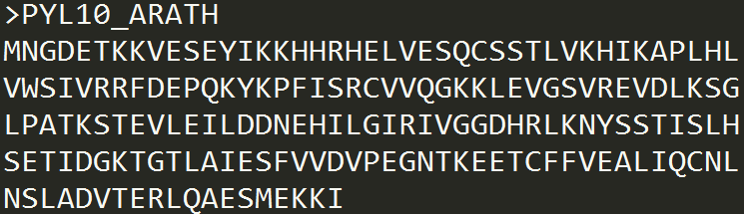
\includegraphics{figures/fasta_pyl10_ara.png}
\caption{\label{fig:fastaPYL}Protein sequence of PYL10 in Arabidopsis.}
\end{figure}

\begin{Shaded}
\begin{Highlighting}[]
\KeywordTok{#!/usr/bin/perl}
\FunctionTok{use} \KeywordTok{warnings}\NormalTok{;}
\FunctionTok{use} \KeywordTok{strict}\NormalTok{;}

\KeywordTok{my} \DataTypeTok{$fasta}\NormalTok{ = }\KeywordTok{"}\StringTok{./data/test_ref.fa}\KeywordTok{"}\NormalTok{;}

\FunctionTok{open}\NormalTok{ FASTA, }\DataTypeTok{$fasta} \KeywordTok{or} \FunctionTok{die} \KeywordTok{"}\DataTypeTok{$!}\StringTok{: }\DataTypeTok{$fasta}\KeywordTok{"}\NormalTok{;}
\CommentTok{# Set the input record separator}
\DataTypeTok{$/}\NormalTok{ = }\KeywordTok{"}\CharTok{\textbackslash{}n}\StringTok{>}\KeywordTok{"}\NormalTok{;}
\CommentTok{# Print header}
\FunctionTok{print} \KeywordTok{"}\StringTok{Chrom}\CharTok{\textbackslash{}t}\StringTok{Length}\CharTok{\textbackslash{}n}\KeywordTok{"}\NormalTok{;}
\KeywordTok{while}\NormalTok{(}\KeywordTok{my} \DataTypeTok{$chunk}\NormalTok{ = }\KeywordTok{<FASTA>}\NormalTok{)\{}
    \CommentTok{# Remove > in the first chunk}
    \DataTypeTok{$chunk}\NormalTok{ =~ }\KeywordTok{s/}\CharTok{^}\OtherTok{>//;}
\CommentTok{    # Remove \textbackslash{}n> from the end of the chunk}
\OtherTok{    chomp }\DataTypeTok{$chunk}\OtherTok{;}
\CommentTok{    # Assign ID and seq to two variables}
\OtherTok{    my }\CharTok{(}\DataTypeTok{$chrom}\OtherTok{, }\DataTypeTok{$seq}\CharTok{)}\OtherTok{ = split}\CharTok{(}\OtherTok{/}\BaseNTok{\textbackslash{}n}\OtherTok{/, }\DataTypeTok{$chunk}\OtherTok{, 2}\CharTok{)}\OtherTok{;}
\CommentTok{    # Remove \textbackslash{}n in the string}
\OtherTok{    }\DataTypeTok{$seq}\OtherTok{ =~ s/}\BaseNTok{\textbackslash{}n}\OtherTok{//g;}
\CommentTok{    # Calculate the length of sequence.}
\OtherTok{    my }\DataTypeTok{$seq_length}\OtherTok{ = length }\DataTypeTok{$seq}\OtherTok{;}
\CommentTok{    # Print ID and length of the sequence.}
\OtherTok{    print "}\DataTypeTok{$chrom}\OtherTok{\textbackslash{}t}\DataTypeTok{$seq_length}\BaseNTok{\textbackslash{}n}\OtherTok{";}
\OtherTok{\}}
\OtherTok{close FASTA;}
\end{Highlighting}
\end{Shaded}

You can consider the content in the fasta file as a string (Figure
\ref{fig:fastaString}) sperarated by
\texttt{\textbackslash{}n\textgreater{}}.

We set the input record separator \texttt{\$/} as
\texttt{\textbackslash{}n\textgreater{}}.

In the first cycle of the \texttt{while} loop, the first chunk is
\texttt{\textgreater{}chr1\textbackslash{}nACGCTAGCTAGTCAGTCGATCGT\textbackslash{}nCGTAGCTAGCTAG\textbackslash{}n\textgreater{}}.

You should notice that there is a leading \texttt{\textgreater{}} in the
first chunk. So you need to use \texttt{s/\^{}\textgreater{}//} to
remove the leading \texttt{\textgreater{}}.

To remove the trailing \texttt{\textbackslash{}n\textgreater{}}, you can
use \texttt{chomp\ \$chunk;}. Then the string is:

\begin{verbatim}
chr1\nACGCTAGCTAGTCAGTCGATCGT\nCGTAGCTAGCTAG
\end{verbatim}

The string before first \texttt{\textbackslash{}n} is the sequence ID.
The string after the first \texttt{\textbackslash{}n} is the sequence.
To get the sequnce ID and sequnce and assign to two variables, you can
use \texttt{split(/\textbackslash{}n/,\ \$chunk,\ 2)}. Here LIMIT is set
to 2, it represents the maximum number (here 2) of fields into which the
EXPR may be split.

The goal of this code is to output the sequence IDs and their lengths.
Currently the string of the variable (\texttt{\$seq}) is
\texttt{ACGCTAGCTAGTCAGTCGATCGT\textbackslash{}nCGTAGCTAGCTAG}. To do
this, you first need to remove \texttt{\textbackslash{}n} in the
sequence by using
\texttt{\$seq\ =\textasciitilde{}\ s/\textbackslash{}n//g;}. Now the
string of the variable (\texttt{\$seq}) is
\texttt{ACGCTAGCTAGTCAGTCGATCGTCGTAGCTAGCTAG}. Then built-in function
\texttt{length} can be used to calculate the length of the sequence. The
function \texttt{print} is used to output the sequnce ID and the length
of the sequence.

In the second cycles of the \texttt{while} loop, the chunk is
\texttt{chr2\textbackslash{}nCTGCGGGCTAAATCGATCGATCG\textbackslash{}nGTACGTACGAGCTAGCTA\textbackslash{}n\textgreater{}}.

Unlike the first chunk, there is no leading \texttt{\textgreater{}} in
the second chunk. So the code \texttt{s/\^{}\textgreater{}//} will do
nothing for the second chunk.

The following steps is the same as you can do for the first cycle.

In the third cycle of the \texttt{while} loop, you can do the same thing
on the third sequence.



\begin{figure}
\centering
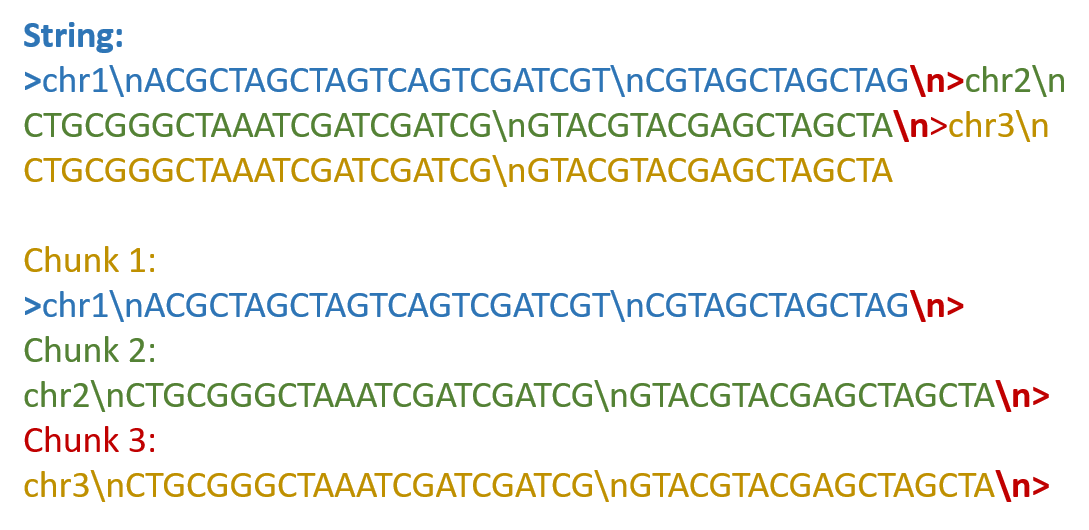
\includegraphics{figures/fasta_string.png}
\caption{\label{fig:fastaString}Fasta string.}
\end{figure}

\begin{Shaded}
\begin{Highlighting}[]
\FunctionTok{perl}\NormalTok{ code_perl/fa_seq_len.pl}
\end{Highlighting}
\end{Shaded}

\begin{verbatim}
## Chrom    Length
## chr1 36
## chr2 41
## chr3 41
\end{verbatim}

\section{Output to a file on the
disk}\label{output-to-a-file-on-the-disk}

\begin{Shaded}
\begin{Highlighting}[]
\KeywordTok{#!/usr/bin/perl}
\FunctionTok{use} \KeywordTok{warnings}\NormalTok{;}
\FunctionTok{use} \KeywordTok{strict}\NormalTok{;}

\KeywordTok{my} \DataTypeTok{$fasta}\NormalTok{   = }\KeywordTok{"}\StringTok{./data/test_ref.fa}\KeywordTok{"}\NormalTok{;}
\KeywordTok{my} \DataTypeTok{$out_len}\NormalTok{ = }\KeywordTok{"}\StringTok{./data/test_ref_len.txt}\KeywordTok{"}\NormalTok{;}

\FunctionTok{open}\NormalTok{ FASTA, }\DataTypeTok{$fasta} \KeywordTok{or} \FunctionTok{die} \KeywordTok{"}\StringTok{Can't open file for reading: }\DataTypeTok{$!}\StringTok{ }\DataTypeTok{$fasta}\KeywordTok{"}\NormalTok{;}
\FunctionTok{open}\NormalTok{ OUT, }\KeywordTok{"}\StringTok{+>}\DataTypeTok{$out_len}\KeywordTok{"} \KeywordTok{or} \FunctionTok{die} \KeywordTok{"}\StringTok{Can't open file for writing: }\DataTypeTok{$!}\StringTok{ }\DataTypeTok{$out_len}\KeywordTok{"}\NormalTok{;}
\CommentTok{# Set the input record separator}
\DataTypeTok{$/}\NormalTok{ = }\KeywordTok{"}\CharTok{\textbackslash{}n}\StringTok{>}\KeywordTok{"}\NormalTok{;}
\CommentTok{# Print header}
\FunctionTok{print}\NormalTok{ OUT }\KeywordTok{"}\StringTok{Chrom}\CharTok{\textbackslash{}t}\StringTok{Length}\CharTok{\textbackslash{}n}\KeywordTok{"}\NormalTok{;}
\KeywordTok{while}\NormalTok{(}\KeywordTok{my} \DataTypeTok{$chunk}\NormalTok{ = }\KeywordTok{<FASTA>}\NormalTok{)\{}
    \CommentTok{# Remove > in the first chunk}
    \DataTypeTok{$chunk}\NormalTok{ =~ }\KeywordTok{s/}\CharTok{^}\OtherTok{>//;}
\CommentTok{    # Remove \textbackslash{}n> from the end of the chunk}
\OtherTok{    chomp }\DataTypeTok{$chunk}\OtherTok{;}
\CommentTok{    # Assign ID and seq to two variables}
\OtherTok{    my }\CharTok{(}\DataTypeTok{$chrom}\OtherTok{, }\DataTypeTok{$seq}\CharTok{)}\OtherTok{ = split}\CharTok{(}\OtherTok{/}\BaseNTok{\textbackslash{}n}\OtherTok{/, }\DataTypeTok{$chunk}\OtherTok{, 2}\CharTok{)}\OtherTok{;}
\CommentTok{    # Remove \textbackslash{}n in the string}
\OtherTok{    }\DataTypeTok{$seq}\OtherTok{ =~ s/}\BaseNTok{\textbackslash{}n}\OtherTok{//g;}
\CommentTok{    # Calculate the length of sequence.}
\OtherTok{    my }\DataTypeTok{$seq_length}\OtherTok{ = length }\DataTypeTok{$seq}\OtherTok{;}
\CommentTok{    # Print ID and length of the sequence.}
\OtherTok{    print OUT "}\DataTypeTok{$chrom}\OtherTok{\textbackslash{}t}\DataTypeTok{$seq_length}\BaseNTok{\textbackslash{}n}\OtherTok{";}
\OtherTok{\}}
\OtherTok{close FASTA;}
\OtherTok{close OUT;}
\end{Highlighting}
\end{Shaded}

\begin{Shaded}
\begin{Highlighting}[]
\FunctionTok{perl}\NormalTok{ code_perl/fa_seq_len_out.pl}
\FunctionTok{cat}\NormalTok{ ./data/test_ref_len.txt}
\end{Highlighting}
\end{Shaded}

\begin{verbatim}
## Chrom    Length
## chr1 36
## chr2 41
## chr3 41
\end{verbatim}

\section{Arguments from command line}\label{arguments-from-command-line}

Imagine you have 5 fasta files and you want to calculate sequence
lengths for all the 5 files, if you modify the file each time you run
the code, it will be very tedious.

Perls provides an array called \texttt{@ARGV}. \texttt{@ARGV} holds all
the arguments from the command line. The first one will be
\texttt{\$ARGV{[}0{]}}.

\texttt{@ARGV} will automatically hold all the arguments. If no
arguments are provided, \texttt{@ARGV} will be empty.

The following example shows you how it looks like in real code.

\begin{Shaded}
\begin{Highlighting}[]
\KeywordTok{#!/usr/bin/perl}
\FunctionTok{use} \KeywordTok{warnings}\NormalTok{;}
\FunctionTok{use} \KeywordTok{strict}\NormalTok{;}

\KeywordTok{my}\NormalTok{ (}\DataTypeTok{$fasta}\NormalTok{, }\DataTypeTok{$out_len}\NormalTok{) = }\DataTypeTok{@ARGV}\NormalTok{; }
\FunctionTok{print} \KeywordTok{"}\StringTok{First arguments \textbackslash{}$ARGV[0] : }\DataTypeTok{$ARGV}\StringTok{[0]}\CharTok{\textbackslash{}n}\KeywordTok{"}\NormalTok{;}
\FunctionTok{print} \KeywordTok{"}\StringTok{Second arguments \textbackslash{}$ARGV[0]: }\DataTypeTok{$ARGV}\StringTok{[1]}\CharTok{\textbackslash{}n}\KeywordTok{"}\NormalTok{;}

\FunctionTok{print} \KeywordTok{"}\StringTok{The variable \textbackslash{}$fasta:   }\DataTypeTok{$fasta}\CharTok{\textbackslash{}n}\KeywordTok{"}\NormalTok{;}
\FunctionTok{print} \KeywordTok{"}\StringTok{The variable \textbackslash{}$out_len: }\DataTypeTok{$out_len}\CharTok{\textbackslash{}n}\KeywordTok{"}\NormalTok{;}
\end{Highlighting}
\end{Shaded}

\begin{Shaded}
\begin{Highlighting}[]
\FunctionTok{perl}\NormalTok{ code_perl/test_argv.pl test_ref.fa test_ref_len.txt}
\end{Highlighting}
\end{Shaded}

\begin{verbatim}
## First arguments $ARGV[0] : test_ref.fa
## Second arguments $ARGV[0]: test_ref_len.txt
## The variable $fasta:   test_ref.fa
## The variable $out_len: test_ref_len.txt
\end{verbatim}

In the above example, the first argument is \texttt{\$ARGV{[}0{]}} which
stores the file name: test\_ref.fa. The second one stores the file name:
test\_ref\_len.txt. It's highly recommended to assign the values in
\texttt{@ARGV} to some variables that the readers (including yourself)
can understand the variables based on the names.

Here I'll show you how to use ARGV using an example. The code below will
show you what to do if you want to filter a fasta file based on the
sequence length.

\begin{Shaded}
\begin{Highlighting}[]
\KeywordTok{#!/usr/bin/perl}
\FunctionTok{use} \KeywordTok{warnings}\NormalTok{;}
\FunctionTok{use} \KeywordTok{strict}\NormalTok{;}

\KeywordTok{my}\NormalTok{ (}\DataTypeTok{$fasta}\NormalTok{, }\DataTypeTok{$out_len}\NormalTok{) = }\DataTypeTok{@ARGV}\NormalTok{; }

\FunctionTok{open}\NormalTok{ FASTA, }\DataTypeTok{$fasta} \KeywordTok{or} \FunctionTok{die} \KeywordTok{"}\StringTok{Can't open file for reading: }\DataTypeTok{$!}\StringTok{ }\DataTypeTok{$fasta}\KeywordTok{"}\NormalTok{;}
\FunctionTok{open}\NormalTok{ OUT, }\KeywordTok{"}\StringTok{+>}\DataTypeTok{$out_len}\KeywordTok{"} \KeywordTok{or} \FunctionTok{die} \KeywordTok{"}\StringTok{Can't open file for writing: }\DataTypeTok{$!}\StringTok{ }\DataTypeTok{$out_len}\KeywordTok{"}\NormalTok{;}
\CommentTok{# Set the input record separator}
\DataTypeTok{$/}\NormalTok{ = }\KeywordTok{"}\CharTok{\textbackslash{}n}\StringTok{>}\KeywordTok{"}\NormalTok{;}
\CommentTok{# Print header}
\FunctionTok{print}\NormalTok{ OUT }\KeywordTok{"}\StringTok{The input file name is: }\DataTypeTok{$fasta}\CharTok{\textbackslash{}n}\KeywordTok{"}\NormalTok{;}
\FunctionTok{print}\NormalTok{ OUT }\KeywordTok{"}\StringTok{Chrom}\CharTok{\textbackslash{}t}\StringTok{Length}\CharTok{\textbackslash{}n}\KeywordTok{"}\NormalTok{;}
\KeywordTok{while}\NormalTok{(}\KeywordTok{my} \DataTypeTok{$chunk}\NormalTok{ = }\KeywordTok{<FASTA>}\NormalTok{)\{}
    \CommentTok{# Remove > in the first chunk}
    \DataTypeTok{$chunk}\NormalTok{ =~ }\KeywordTok{s/}\CharTok{^}\OtherTok{>//;}
\CommentTok{    # Remove \textbackslash{}n> from the end of the chunk}
\OtherTok{    chomp }\DataTypeTok{$chunk}\OtherTok{;}
\CommentTok{    # Assign ID and seq to two variables}
\OtherTok{    my }\CharTok{(}\DataTypeTok{$chrom}\OtherTok{, }\DataTypeTok{$seq}\CharTok{)}\OtherTok{ = split}\CharTok{(}\OtherTok{/}\BaseNTok{\textbackslash{}n}\OtherTok{/, }\DataTypeTok{$chunk}\OtherTok{, 2}\CharTok{)}\OtherTok{;}
\CommentTok{    # Remove \textbackslash{}n in the string}
\OtherTok{    }\DataTypeTok{$seq}\OtherTok{ =~ s/}\BaseNTok{\textbackslash{}n}\OtherTok{//g;}
\CommentTok{    # Calculate the length of sequence.}
\OtherTok{    my }\DataTypeTok{$seq_length}\OtherTok{ = length }\DataTypeTok{$seq}\OtherTok{;}
\CommentTok{    # Print ID and length of the sequence.}
\OtherTok{    print OUT "}\DataTypeTok{$chrom}\OtherTok{\textbackslash{}t}\DataTypeTok{$seq_length}\BaseNTok{\textbackslash{}n}\OtherTok{";}
\OtherTok{\}}
\OtherTok{close FASTA;}
\OtherTok{close OUT;}
\end{Highlighting}
\end{Shaded}

For example if you want to remove the sequences that is shorter than 30
bps, you can use the following example.

\begin{Shaded}
\begin{Highlighting}[]
\BuiltInTok{printf} \StringTok{"Before filtering:\textbackslash{}n"}
\FunctionTok{cat}\NormalTok{ ./data/test_ref2.fa}
\FunctionTok{perl}\NormalTok{ code_perl/fa_seq_len_out_argv_fil.pl ./data/test_ref2.fa 30 ./data/test_ref2_30.fa}

\BuiltInTok{printf} \StringTok{"\textbackslash{}nAfter filtering: \textbackslash{}n"}
\FunctionTok{cat}\NormalTok{ ./data/test_ref2_30.fa }
\end{Highlighting}
\end{Shaded}

\begin{verbatim}
## Before filtering:
## >chr1
## ACGCTAGCTAGTCAGTCGATCGT
## CGTAGCTAGCTAG
## >chr2
## CTGCGGGCTAAATCGATCGATCG
## GTACGTACGAGCTAGCTAA
## >chr3
## CTGCGGGCTAAATCGATCGATCG
## GTACGTACGAG
## >chr4
## CTGCGGGCTAAATCAGCTAA
## >chr5
## CTGCTCGATCGATCGACGAGCTA
## GCTA
## After filtering: 
## The input file name is: ./data/test_ref2.fa
## Chrom    Length
## >chr1 36
## ACGCTAGCTAGTCAGTCGATCGTCGTAGCTAGCTAG
## >chr2 42
## CTGCGGGCTAAATCGATCGATCGGTACGTACGAGCTAGCTAA
## >chr3 34
## CTGCGGGCTAAATCGATCGATCGGTACGTACGAG
\end{verbatim}

If you have multiple files, you can just change the file names in the
command line. It's very handy. You can also change the length cutoff in
the command line.

\chapter{Perl modules}\label{perl-modules}

\section{What is a Perl module}\label{what-is-a-perl-module}

Perl modules are a set of related functions in a library file. They are
specifically designed to be reusable by other modules or programs. There
are more than 100,000 modules ready for you to use on the Comprehensive
Perl Archive Network.

Most Perl modules are written in Perl, some use XS (they are written in
C) so require a C compiler. Modules may have dependencies on other
modules (almost always on CPAN) and cannot be installed without them (or
without a specific version of them). Many modules on CPAN now require a
recent version of Perl (version 5.8 or above).

The reason that we need to use Perl module is Perl module can largely
reduce our coding work.

\section{How to install a Perl
module}\label{how-to-install-a-perl-module}

Here we'll only discuss how to install Perl module in Linux system. The
easies way I think is to use \texttt{cpanm}.

Here is how you can do this. First go to webpage and download the
\texttt{cpanm} source code.

\begin{verbatim}
## Web link:https://raw.githubusercontent.com/miyagawa/cpanminus/master/cpanm

chmod 755 cpanm

./cpanm Bio::Seq
\end{verbatim}

NOTE

\BeginKnitrBlock{rmdtip}
\textbf{Possible problem when using \texttt{cpanm}}

You may encouter the following error message. This is a bug from Perl.
You cna run \texttt{yum\ install\ perl-CPAN} resolved the issue.

Here is the ERROR MESSAGE:

! ! Can't write to /usr/local/share/perl5 and /usr/local/bin: Installing
modules to /home/xie186/perl5 ! To turn off this warning, you have to do
one of the following: ! - run me as a root or with --sudo option (to
install to /usr/local/share/perl5 and /usr/local/bin) ! - Configure
local::lib in your existing shell to set PERL\_MM\_OPT etc. ! - Install
local::lib by running the following commands ! ! cpanm
--local-lib=\textasciitilde{}/perl5 local::lib \&\& eval \$(perl -I
\textasciitilde{}/perl5/lib/perl5/ -Mlocal::lib) ! --\textgreater{}
Working on Bio::Seq Fetching
\url{http://www.cpan.org/authors/id/C/CJ/CJFIELDS/BioPerl-1.007001.tar.gz}
\ldots{} OK ==\textgreater{} Found dependencies: Module::Build,
ExtUtils::Install --\textgreater{} Working on Module::Build Fetching
\url{http://www.cpan.org/authors/id/L/LE/LEONT/Module-Build-0.4222.tar.gz}
\ldots{} OK ==\textgreater{} Found dependencies: Module::Metadata,
version, CPAN::Meta, Perl::OSType --\textgreater{} Working on
Module::Metadata Fetching
\url{http://www.cpan.org/authors/id/E/ET/ETHER/Module-Metadata-1.000033.tar.gz}
\ldots{} OK ==\textgreater{} Found dependencies: ExtUtils::MakeMaker
--\textgreater{} Working on ExtUtils::MakeMaker Fetching
\url{http://www.cpan.org/authors/id/B/BI/BINGOS/ExtUtils-MakeMaker-7.26.tar.gz}
\ldots{} OK Configuring ExtUtils-MakeMaker-7.26 \ldots{} OK Can't locate
ExtUtils/Manifest.pm in \citet{INC} (\citet{INC} contains:
FatPacked::26160008=HASH(0x18f2b88) /usr/local/lib64/perl5
/usr/local/share/perl5 /usr/lib64/perl5/vendor\_perl
/usr/share/perl5/vendor\_perl /usr/lib64/perl5 /usr/share/perl5 .) at
./cpanm line 132.
\EndKnitrBlock{rmdtip}

\section{How to use a Perl module}\label{how-to-use-a-perl-module}

\section{How to use BioPerl module}\label{how-to-use-bioperl-module}

\section{How to write a module}\label{how-to-write-a-module}

The name \texttt{R} is partly based on the (first) names of the first
two R authors (Robert Gentleman and Ross Ihaka).

Convert string to a variable name
\url{https://stackoverflow.com/questions/6034655/convert-string-to-a-variable-name}

\begin{verbatim}
assign("x", 5)

x
[1] 5
\end{verbatim}

\url{https://cran.r-project.org/doc/FAQ/R-FAQ.html\#Why-is-R-named-R_003f}

\chapter{Producing simple graphs}\label{producing-simple-graphs}

\section{Producing simple graphs using
R}\label{producing-simple-graphs-using-r}

\subsection{Line Charts}\label{line-charts}

\subsection{Bar Charts}\label{bar-charts}

\subsection{Histograms}\label{histograms}

\subsection{Pie Charts}\label{pie-charts}

\subsection{Dotcharts}\label{dotcharts}

\subsection{Misc}\label{misc}

\chapter{Preparation of figures for
manuscript}\label{preparation-of-figures-for-manuscript}

Inkscape is an open source software which can be used to arrange, crop,
and annotate your images; bring in graphs and charts; draw diagrams; and
export the final figure in whatever format the journal wants.

\section{}\label{section-2}

\chapter{Start a project}\label{start-a-project}

\section{Experimetal design}\label{experimetal-design}

Before

\subsection{How many biological
replicates}\label{how-many-biological-replicates}

\subsection{How big}\label{how-big}

\subsection{How much data to generate}\label{how-much-data-to-generate}

\subsection{}\label{section-3}

Where to start?

There are many ways to start to talk about Bioinformatics analysis. Here
we'll go from whether there is a reference genome or not. Let's take
RNA-seq as an example.

\chapter{Introduction of NGS}\label{introduction-of-ngs}

\section{What is NGS}\label{what-is-ngs}

Genetic information is stored within the chemical structure of the
molecule DNA. DNA can be transcribed into RNA. Then RNA can be
translated into protein.

NGS (Next geneneration sequencing) is not an accurate term. An more
accurate term maybe high throughput sequencing. NGS is specifically used
to refer to sequencing technologies after Sanger sequencing (1st
generation) and single molecular sequencing (3rd sequencing,
e.g.~PacBio) and nanopore based sequencing (4th generation, e.g.~Oxford
Nanopore).

\section{Application of NGS}\label{application-of-ngs}

\section{}\label{section-4}

\section{Usefull links:}\label{usefull-links}

\url{http://www.ecseq.com/support/ngs/trimming-adapter-sequences-is-it-necessary}

\url{http://www.gendx.com/illumina-adapter-ligation-librx}

\url{http://veleta.rosety.com/plasmid.html}

\chapter{Practical Perl program}\label{practical-perl-program}

\section{Extract sequences from genomic DNA for some specific
regions}\label{extract-sequences-from-genomic-dna-for-some-specific-regions}

Figure 8.1 shows how to extract sequences from genomic DNA for some
specific regions. For example, when we perform ChIP-seq for a
transcription factor. We will get the binding sites (some regions) of
transcription factor after analyzing ChIP-seq. You want to know whether
there is motifs that can be recognized by the transcription factor.

The Perl program in Figure 8.1 has two arguments (input files): genomic
DNA sequences and ChIP-seq peak regions. It will print the genomic DNA
sequences for each region in fasta format. We can use
\texttt{\textgreater{}} to generate a new file to record the result
(Figure 8.1).

The genomic DNA sequence data is saved in fasta format (See 11.1).
ChIP-seq peak regions are saved in BED format (See 12.3).

Let's go through each line in detail.

A normal paragraph.

The above code provides an interactive HTML page (figure \ref{fig:foo})




\begin{Shaded}
\begin{Highlighting}[]
\KeywordTok{plot}\NormalTok{(}\DecValTok{1}\NormalTok{)  }\CommentTok{# a scatterplot}
\end{Highlighting}
\end{Shaded}

\begin{figure}
\centering
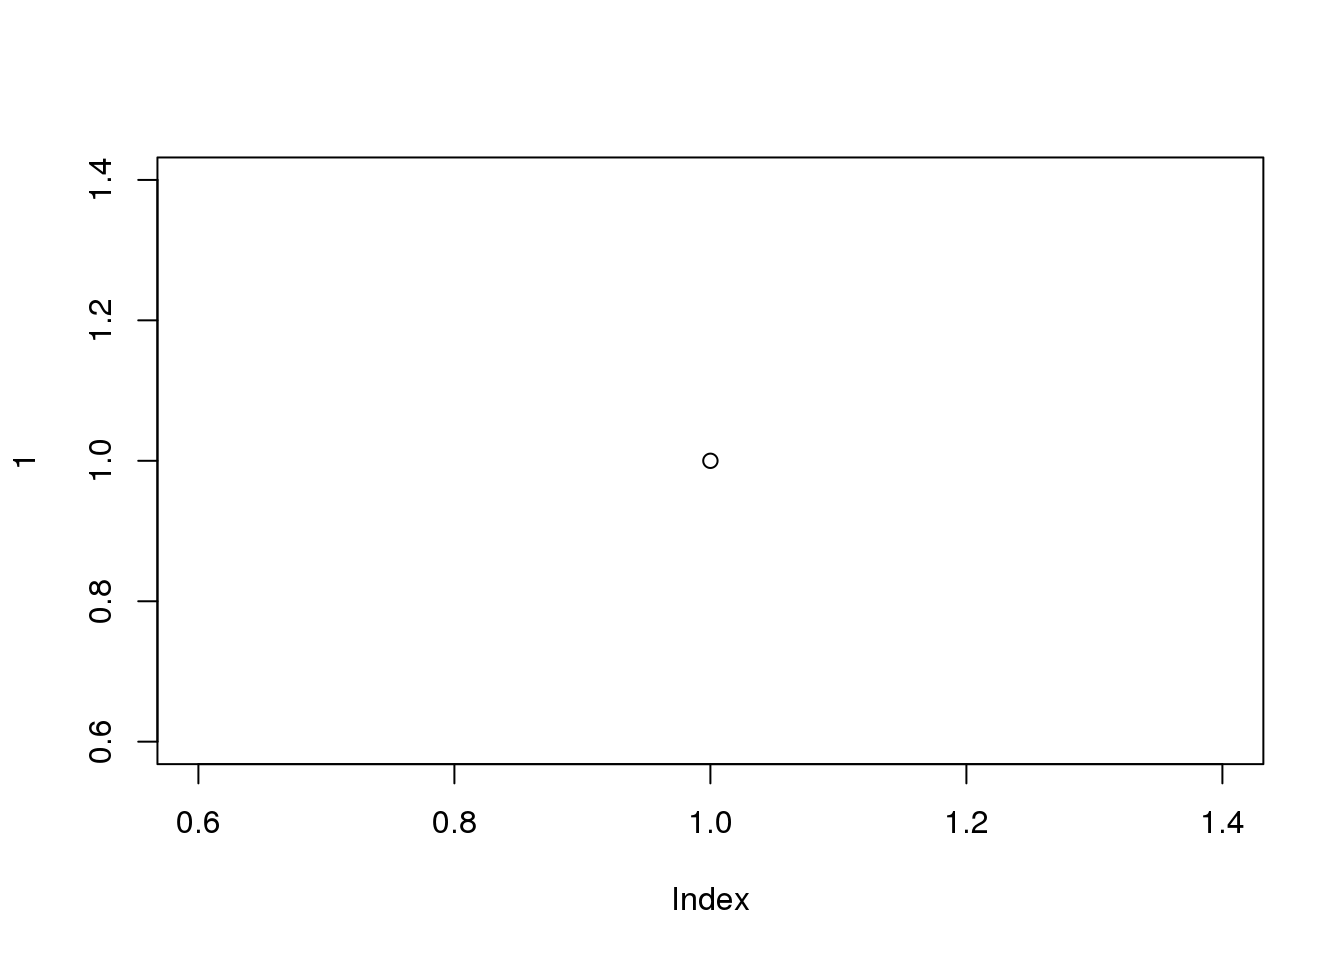
\includegraphics{bioinfBookXIE186_files/figure-latex/foo-1.pdf}
\caption{\label{fig:foo}A scatterplot of the data \texttt{cars} using \textbf{base} R
graphics.}
\end{figure}

\chapter{String manipulation}\label{string-manipulation-1}

\section{String concatenation}\label{string-concatenation-1}

Dot (\texttt{.}) can be used to concatenate two strings together.

\begin{Shaded}
\begin{Highlighting}[]
\CommentTok{# concatenate two strings together and assing to $z}
\DataTypeTok{$z}\NormalTok{ = }\DataTypeTok{$x}\NormalTok{ . }\DataTypeTok{$y}\NormalTok{;}
\CommentTok{# Append $y to $x}
\DataTypeTok{$x}\NormalTok{ = }\DataTypeTok{$x}\NormalTok{ . }\DataTypeTok{$y}\NormalTok{;}
\CommentTok{# Append $y to $x}
\DataTypeTok{$x}\NormalTok{ .= }\DataTypeTok{$y}\NormalTok{;}
\end{Highlighting}
\end{Shaded}

A more convenient way is to use operator \texttt{.=} to append one
variable to another.

As is any other assignments in Perl, if you see an assignment written
this way \$x = \$x op expr, where op stands for any operator and expr
stands for the rest of the statement, you can make a shorter version by
moving the op to the front of the assignment, e.g., \$x op= expr. The
string concatenation operator \texttt{.} is just one possible op among
many others such as \texttt{+}, \texttt{-}, \texttt{*} and \texttt{/}.

\begin{Shaded}
\begin{Highlighting}[]
\DataTypeTok{$x}\NormalTok{ = }\DecValTok{5}\NormalTok{;}
\DataTypeTok{$y}\NormalTok{ = }\DecValTok{6}\NormalTok{;}
\CommentTok{# Append $y to $x}
\DataTypeTok{$x}\NormalTok{ = }\DataTypeTok{$x}\NormalTok{ + }\DataTypeTok{$y}\NormalTok{;}
\CommentTok{# Append $y to $x}
\DataTypeTok{$x}\NormalTok{ += }\DataTypeTok{$y}\NormalTok{;}
\end{Highlighting}
\end{Shaded}

\section{Substring extraction}\label{substring-extraction-1}

\section{Substring search}\label{substring-search-1}

\subsection{index}\label{index}

\subsection{rindex}\label{rindex}

\section{Split String}\label{split-string-1}

\subsection{split}\label{split}

\subsection{join}\label{join}

\subsection{tr}\label{tr}

\subsection{reverse}\label{reverse}

\subsection{markdown}\label{markdown}

\section{Regular expression}\label{regular-expression-1}

\subsection{Pattern matching}\label{pattern-matching-1}

\subsection{Pattern substitution}\label{pattern-substitution-1}

\subsection{Modifiers to pattern matching and
substitution}\label{modifiers-to-pattern-matching-and-substitution-1}

\subsection{Greedy or non-greedy}\label{greedy-or-non-greedy-1}

\subsection{}\label{section-5}

The split function

\chapter{Heatmap Tutorial}\label{heatmap-tutorial}

\href{https://goo.gl/KLZ7N0}{Data link}

\section{\texorpdfstring{Install \texttt{pheatmap}
package}{Install pheatmap package}}\label{install-pheatmap-package}

\begin{verbatim}
install.packages("pheatmap")
\end{verbatim}

\section{Draw a heatmap for gene expression of RNA-seq
data}\label{draw-a-heatmap-for-gene-expression-of-rna-seq-data}

\begin{Shaded}
\begin{Highlighting}[]
\KeywordTok{library}\NormalTok{(pheatmap)}
\NormalTok{gene_exp <-}\StringTok{ }\KeywordTok{read.table}\NormalTok{(}\StringTok{"data/maize_embryo_specific_gene_Sheet1.tsv"}\NormalTok{, }\DataTypeTok{header=}\NormalTok{T, }\DataTypeTok{row.names=}\DecValTok{1}\NormalTok{)}
\KeywordTok{pheatmap}\NormalTok{(gene_exp)}
\end{Highlighting}
\end{Shaded}

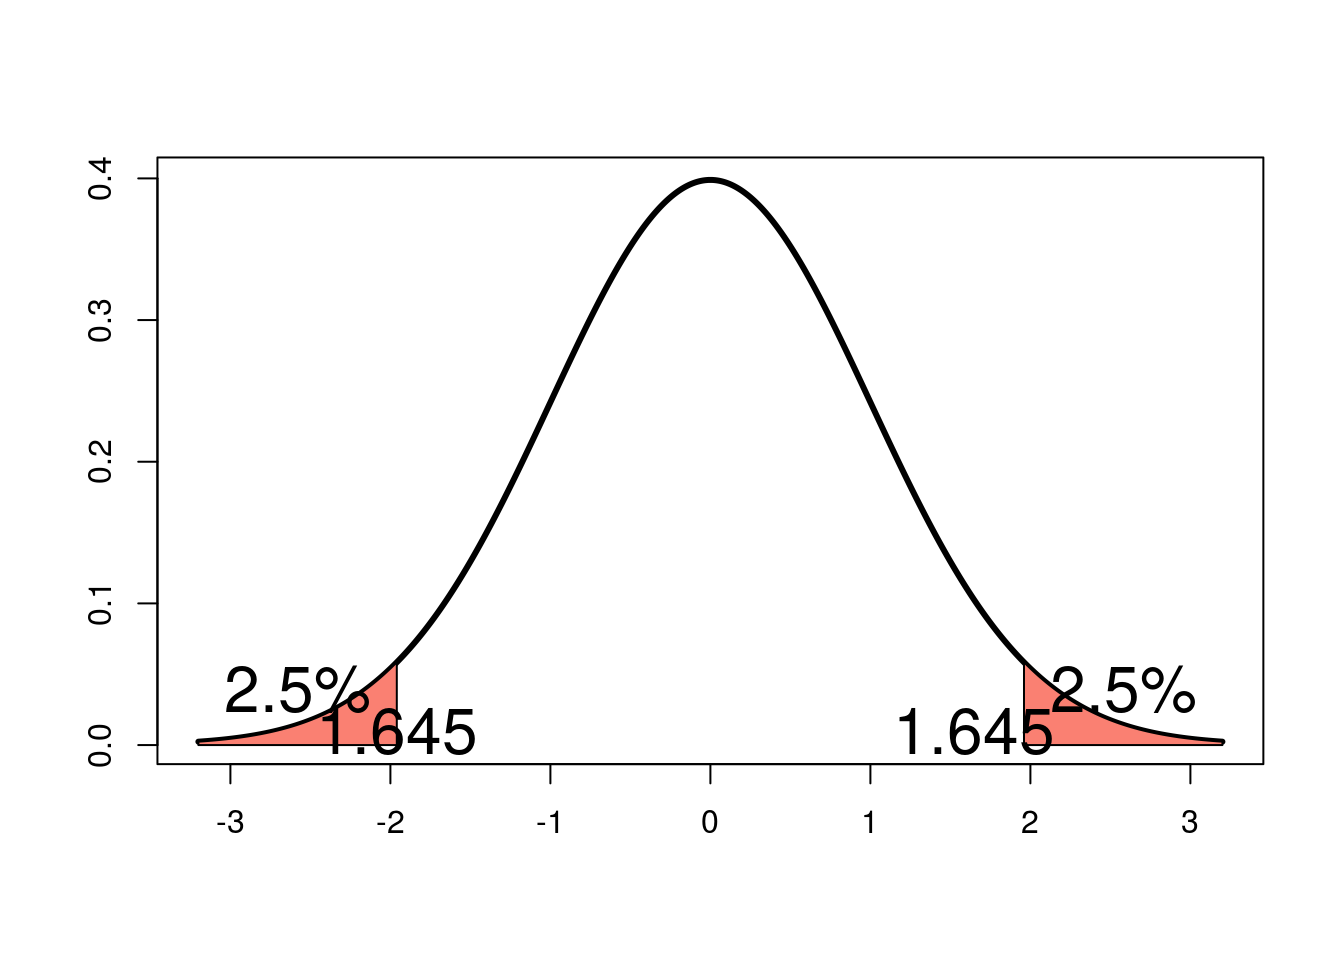
\includegraphics{bioinfBookXIE186_files/figure-latex/unnamed-chunk-64-1.pdf}

\begin{Shaded}
\begin{Highlighting}[]
\KeywordTok{pheatmap}\NormalTok{(}\KeywordTok{log2}\NormalTok{(gene_exp }\OperatorTok{+}\StringTok{ }\FloatTok{0.000001}\NormalTok{), }\DataTypeTok{scale=}\StringTok{"row"}\NormalTok{)}
\end{Highlighting}
\end{Shaded}

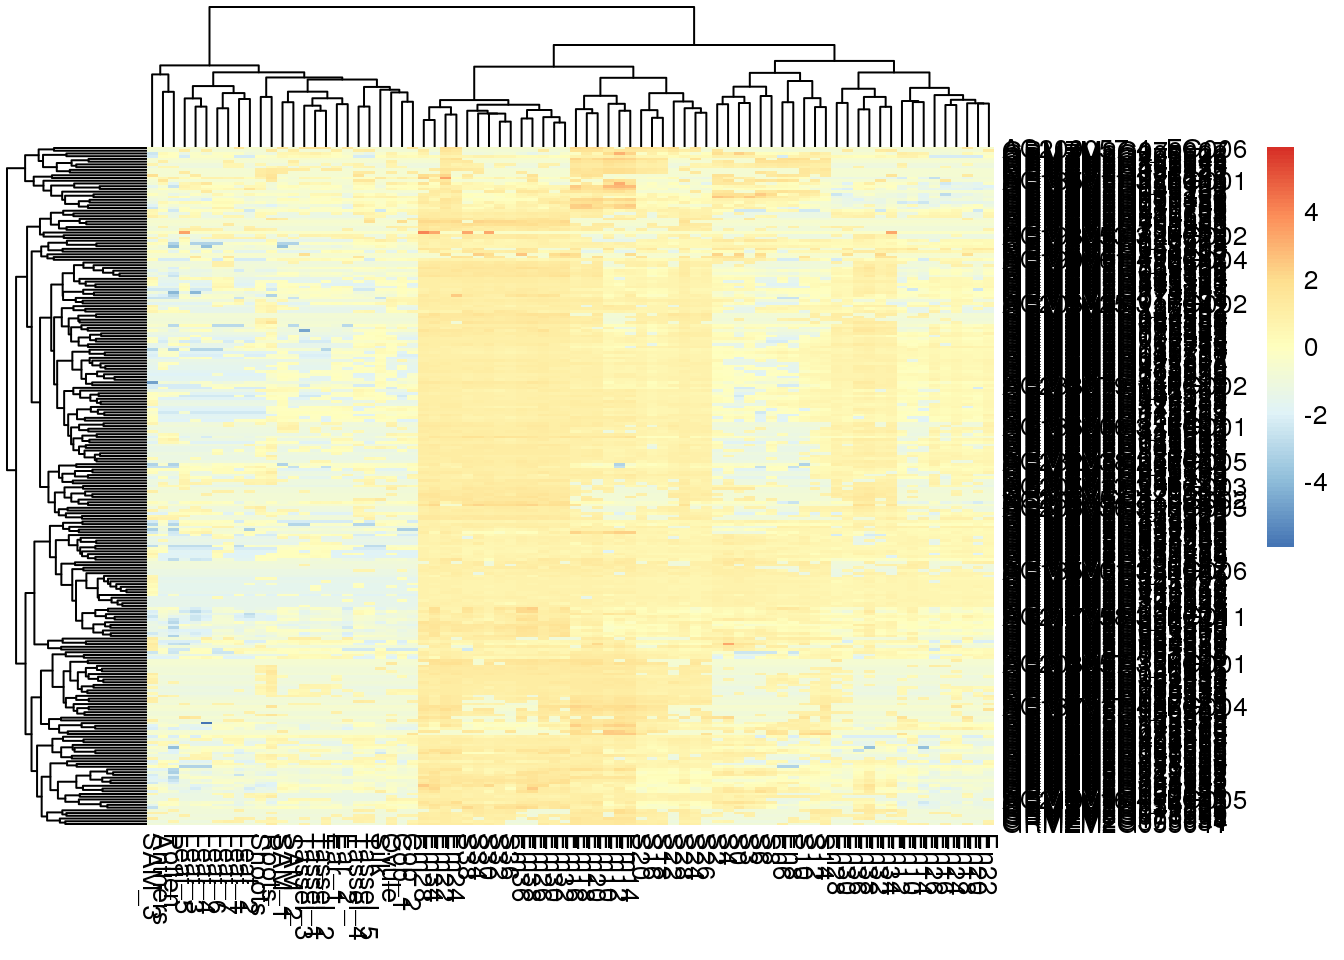
\includegraphics{bioinfBookXIE186_files/figure-latex/unnamed-chunk-64-2.pdf}

\begin{Shaded}
\begin{Highlighting}[]
\KeywordTok{pheatmap}\NormalTok{(}\KeywordTok{log2}\NormalTok{(gene_exp }\OperatorTok{+}\StringTok{ }\FloatTok{0.01}\NormalTok{), }\DataTypeTok{scale=}\StringTok{"row"}\NormalTok{, }\DataTypeTok{show_rownames =}\NormalTok{ T, }\DataTypeTok{show_colnames =}\NormalTok{ F)}
\end{Highlighting}
\end{Shaded}

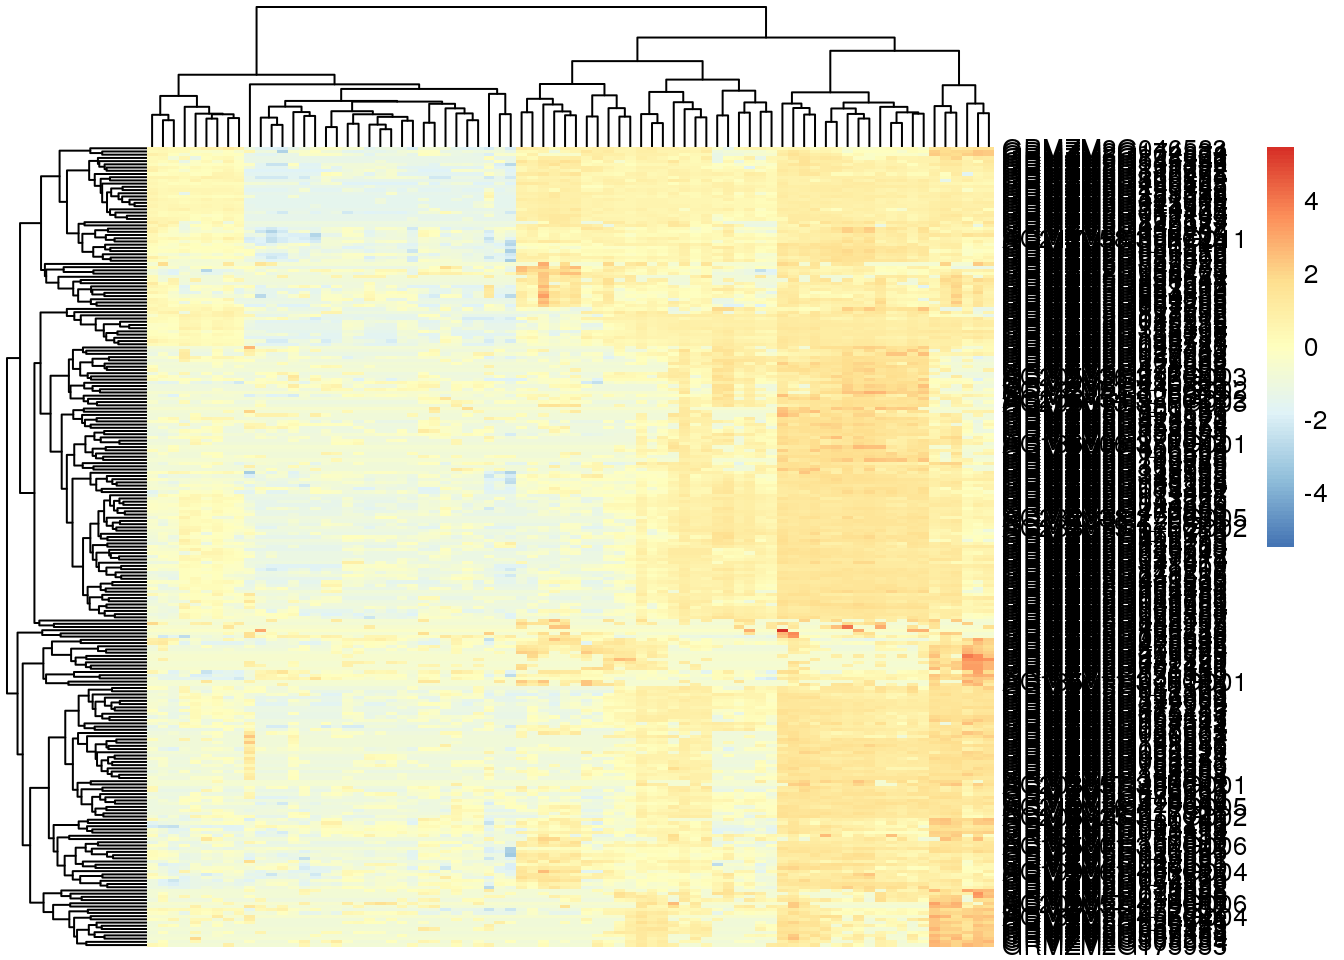
\includegraphics{bioinfBookXIE186_files/figure-latex/unnamed-chunk-64-3.pdf}

\begin{Shaded}
\begin{Highlighting}[]
\KeywordTok{pheatmap}\NormalTok{(}\KeywordTok{log2}\NormalTok{(gene_exp }\OperatorTok{+}\StringTok{ }\FloatTok{0.01}\NormalTok{), }\DataTypeTok{scale=}\StringTok{"row"}\NormalTok{, }\DataTypeTok{show_rownames =}\NormalTok{ F, }\DataTypeTok{show_colnames =}\NormalTok{ T)}
\end{Highlighting}
\end{Shaded}

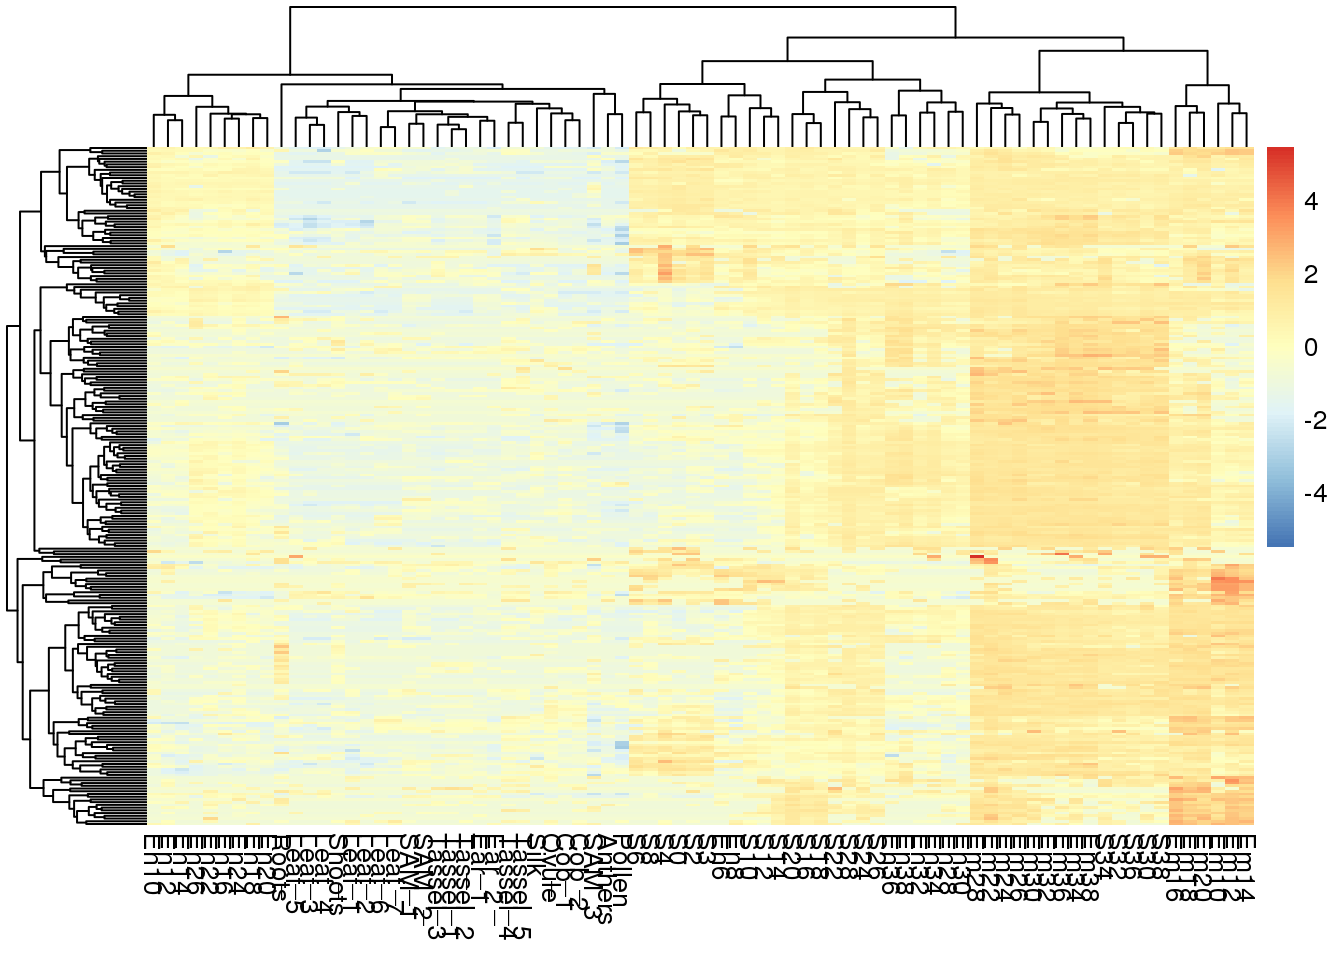
\includegraphics{bioinfBookXIE186_files/figure-latex/unnamed-chunk-64-4.pdf}

\section{Add the annotation}\label{add-the-annotation}

\section{}\label{section-6}

\section{Transfrom the data}\label{transfrom-the-data}

\begin{Shaded}
\begin{Highlighting}[]
\KeywordTok{pheatmap}\NormalTok{(}\KeywordTok{log2}\NormalTok{(gene_exp }\OperatorTok{+}\StringTok{ }\FloatTok{0.01}\NormalTok{)) }
\end{Highlighting}
\end{Shaded}

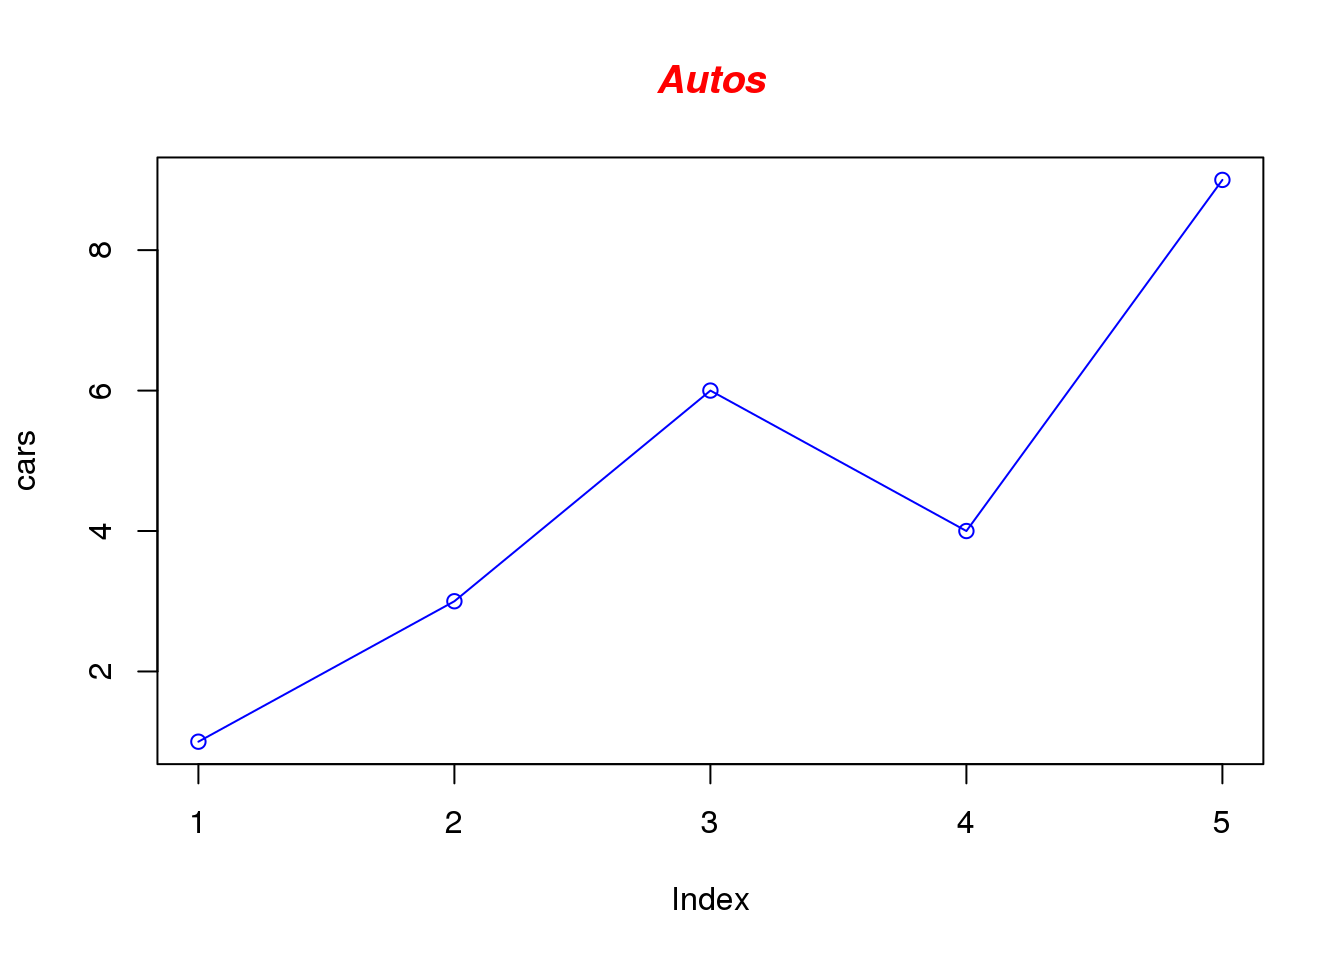
\includegraphics{bioinfBookXIE186_files/figure-latex/unnamed-chunk-65-1.pdf}

\section{How to add annotations}\label{how-to-add-annotations}

\section{How to cut the trees}\label{how-to-cut-the-trees}

\section{How to get the cluster information from the
heatmap}\label{how-to-get-the-cluster-information-from-the-heatmap}

\section{}\label{section-7}

\chapter{Data analysis of RNA-seq}\label{data-analysis-of-rna-seq}

\chapter{BS-seq}\label{bs-seq}

\section{}\label{section-8}

\url{https://www.slideshare.net/secret/Da9IOe8wLsaF8V}

\section{What is BS-seq}\label{what-is-bs-seq}

\section{}\label{section-9}

\section{How to analyze BS-seq data}\label{how-to-analyze-bs-seq-data}

\subsection{}\label{section-10}

MINI REVIEW: Statistical methods for detecting differentially methylated
loci and regions

Strategies for analyzing bisulfite sequencing data

\chapter{Shell}\label{shell}

What is Linux Shell ?

\url{http://www.freeos.com/guides/lsst/}

\chapter{Capstone project:}\label{capstone-project}

\section{Introduction}\label{introduction}

\section{Method}\label{method}

\section{Pipelines}\label{pipelines}

\section{}\label{section-11}

\chapter{Good resouces to learn
Bioinformatics}\label{good-resouces-to-learn-bioinformatics}

\section{References:}\label{references}

\url{https://www.bioinformatics.babraham.ac.uk/training.html}

\chapter{Python}\label{python}

\section{os}\label{os}

\section{}\label{section-12}

\subsection{How to write python script to a command line
program}\label{how-to-write-python-script-to-a-command-line-program}

\url{http://omgenomics.com/python-command-line-program/}

\subsection{Python module: pysam}\label{python-module-pysam}

\subsection{Python module: pybedtools}\label{python-module-pybedtools}

\chapter{R introduction}\label{r-introduction}

\section{Basic R function}\label{basic-r-function}

\section{Producing Simple Graphs with
R}\label{producing-simple-graphs-with-r}

The credit of this section goes to Dr.~Frank McCown
(\citet{simpleGraphR}).

\subsection{Line Charts}\label{line-charts-1}

\begin{Shaded}
\begin{Highlighting}[]
\CommentTok{# Define the cars vector with 5 values}
\NormalTok{cars <-}\StringTok{ }\KeywordTok{c}\NormalTok{(}\DecValTok{1}\NormalTok{, }\DecValTok{3}\NormalTok{, }\DecValTok{6}\NormalTok{, }\DecValTok{4}\NormalTok{, }\DecValTok{9}\NormalTok{)}

\CommentTok{# Graph the cars vector with all defaults}
\KeywordTok{plot}\NormalTok{(cars)}
\end{Highlighting}
\end{Shaded}

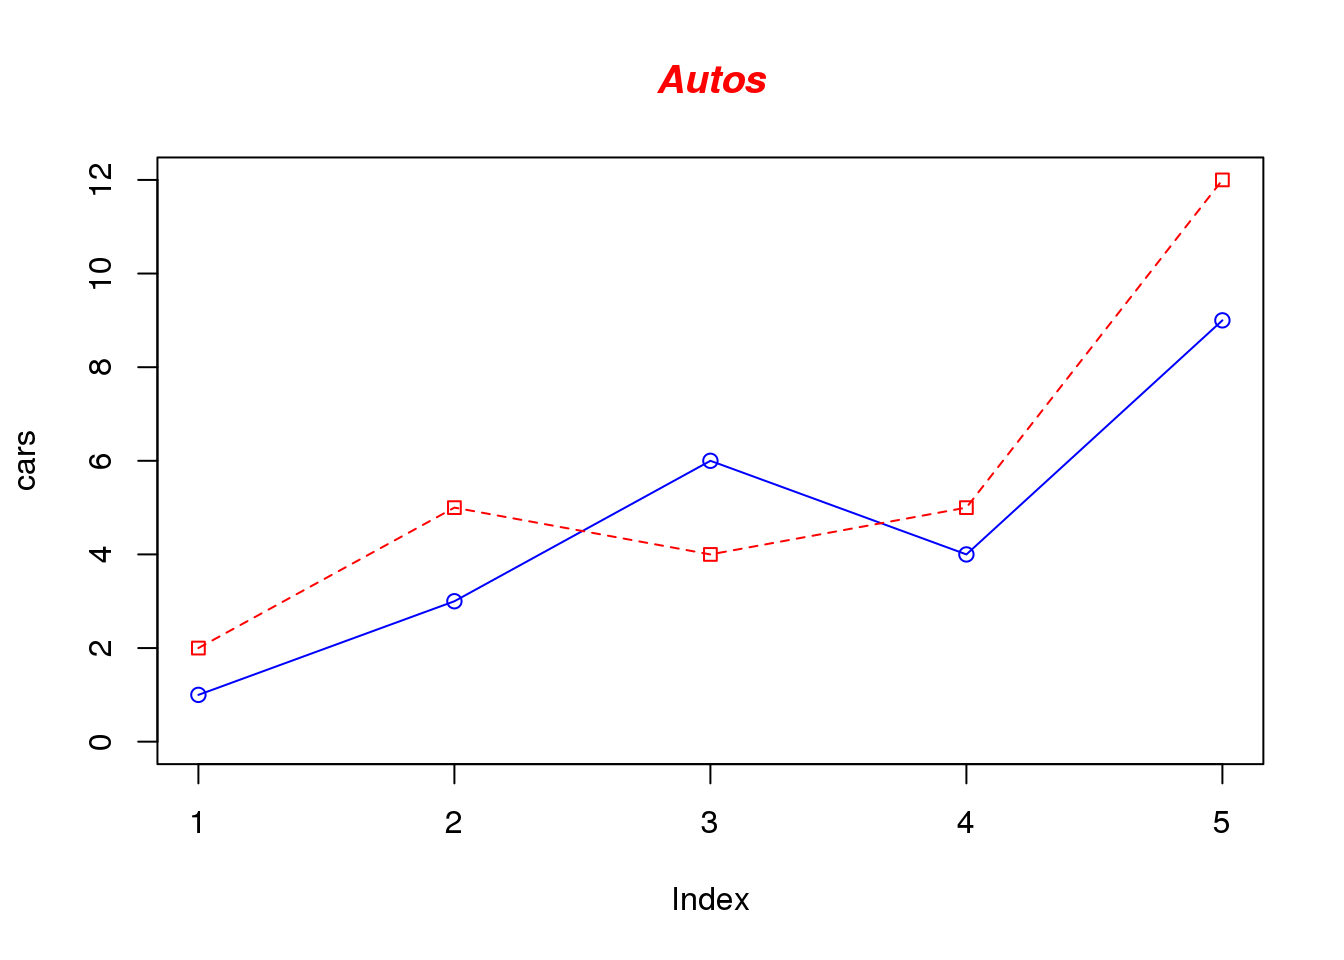
\includegraphics{bioinfBookXIE186_files/figure-latex/unnamed-chunk-66-1.pdf}

\begin{Shaded}
\begin{Highlighting}[]
\NormalTok{?plot}
\end{Highlighting}
\end{Shaded}

Let's add a title, a line to connect the points, and some color:

\begin{Shaded}
\begin{Highlighting}[]
\CommentTok{# Define the cars vector with 5 values}
\NormalTok{cars <-}\StringTok{ }\KeywordTok{c}\NormalTok{(}\DecValTok{1}\NormalTok{, }\DecValTok{3}\NormalTok{, }\DecValTok{6}\NormalTok{, }\DecValTok{4}\NormalTok{, }\DecValTok{9}\NormalTok{)}

\CommentTok{# Graph cars using blue points overlayed by a line }
\KeywordTok{plot}\NormalTok{(cars, }\DataTypeTok{type=}\StringTok{"o"}\NormalTok{, }\DataTypeTok{col=}\StringTok{"blue"}\NormalTok{)}

\CommentTok{# Create a title with a red, bold/italic font}
\KeywordTok{title}\NormalTok{(}\DataTypeTok{main=}\StringTok{"Autos"}\NormalTok{, }\DataTypeTok{col.main=}\StringTok{"red"}\NormalTok{, }\DataTypeTok{font.main=}\DecValTok{4}\NormalTok{)}
\end{Highlighting}
\end{Shaded}

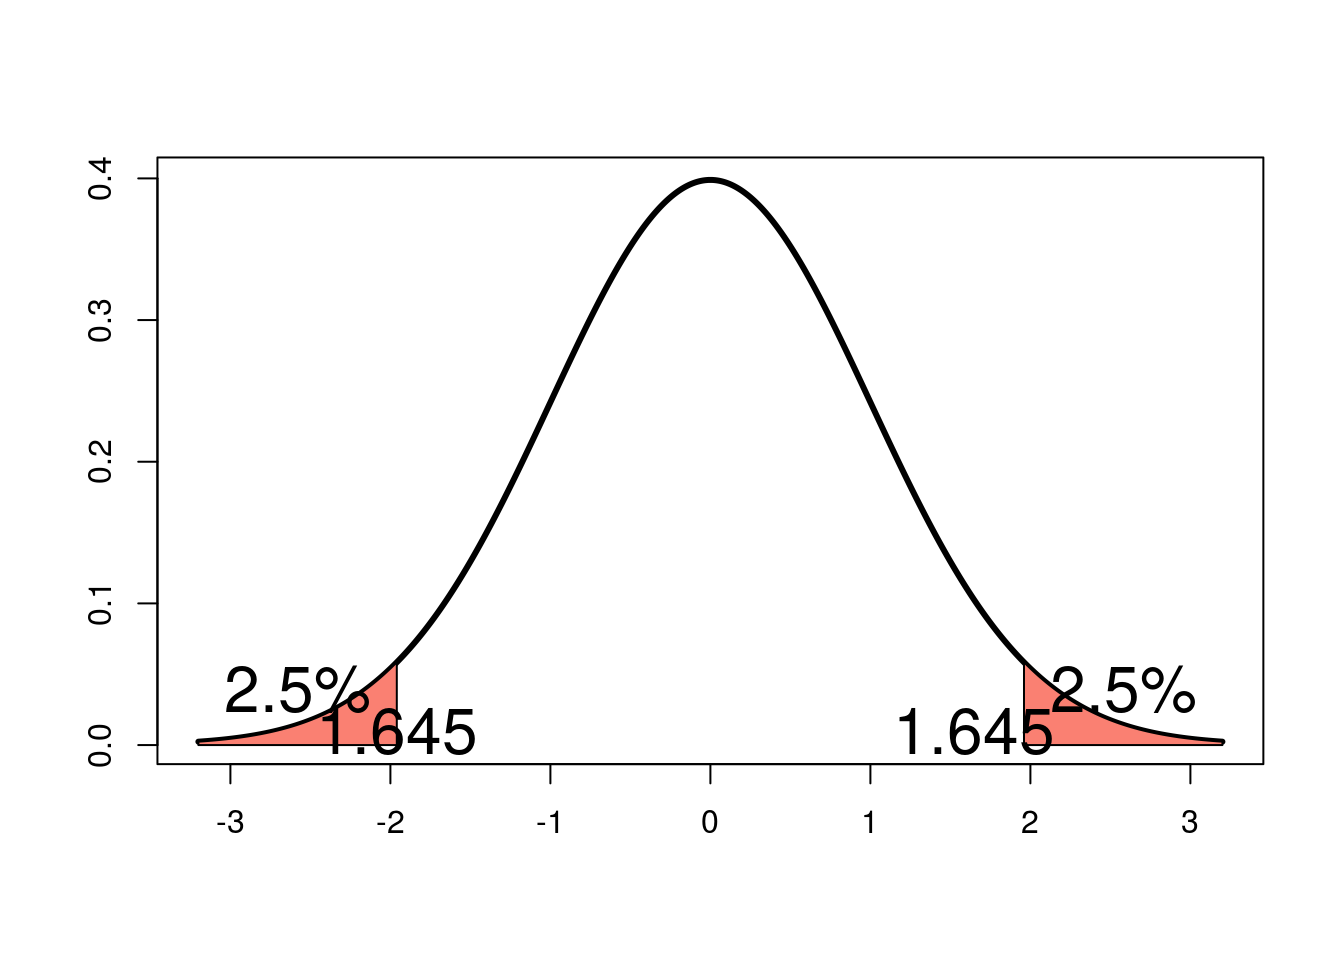
\includegraphics{bioinfBookXIE186_files/figure-latex/unnamed-chunk-67-1.pdf}

Now let's add a red line for trucks and specify the y-axis range
directly so it will be large enough to fit the truck data:

\begin{Shaded}
\begin{Highlighting}[]
\CommentTok{# Define 2 vectors}
\NormalTok{cars <-}\StringTok{ }\KeywordTok{c}\NormalTok{(}\DecValTok{1}\NormalTok{, }\DecValTok{3}\NormalTok{, }\DecValTok{6}\NormalTok{, }\DecValTok{4}\NormalTok{, }\DecValTok{9}\NormalTok{)}
\NormalTok{trucks <-}\StringTok{ }\KeywordTok{c}\NormalTok{(}\DecValTok{2}\NormalTok{, }\DecValTok{5}\NormalTok{, }\DecValTok{4}\NormalTok{, }\DecValTok{5}\NormalTok{, }\DecValTok{12}\NormalTok{)}

\CommentTok{# Graph cars using a y axis that ranges from 0 to 12}
\KeywordTok{plot}\NormalTok{(cars, }\DataTypeTok{type=}\StringTok{"o"}\NormalTok{, }\DataTypeTok{col=}\StringTok{"blue"}\NormalTok{, }\DataTypeTok{ylim=}\KeywordTok{c}\NormalTok{(}\DecValTok{0}\NormalTok{,}\DecValTok{12}\NormalTok{))}

\CommentTok{# Graph trucks with red dashed line and square points}
\KeywordTok{lines}\NormalTok{(trucks, }\DataTypeTok{type=}\StringTok{"o"}\NormalTok{, }\DataTypeTok{pch=}\DecValTok{22}\NormalTok{, }\DataTypeTok{lty=}\DecValTok{2}\NormalTok{, }\DataTypeTok{col=}\StringTok{"red"}\NormalTok{)}

\CommentTok{# Create a title with a red, bold/italic font}
\KeywordTok{title}\NormalTok{(}\DataTypeTok{main=}\StringTok{"Autos"}\NormalTok{, }\DataTypeTok{col.main=}\StringTok{"red"}\NormalTok{, }\DataTypeTok{font.main=}\DecValTok{4}\NormalTok{)}
\end{Highlighting}
\end{Shaded}

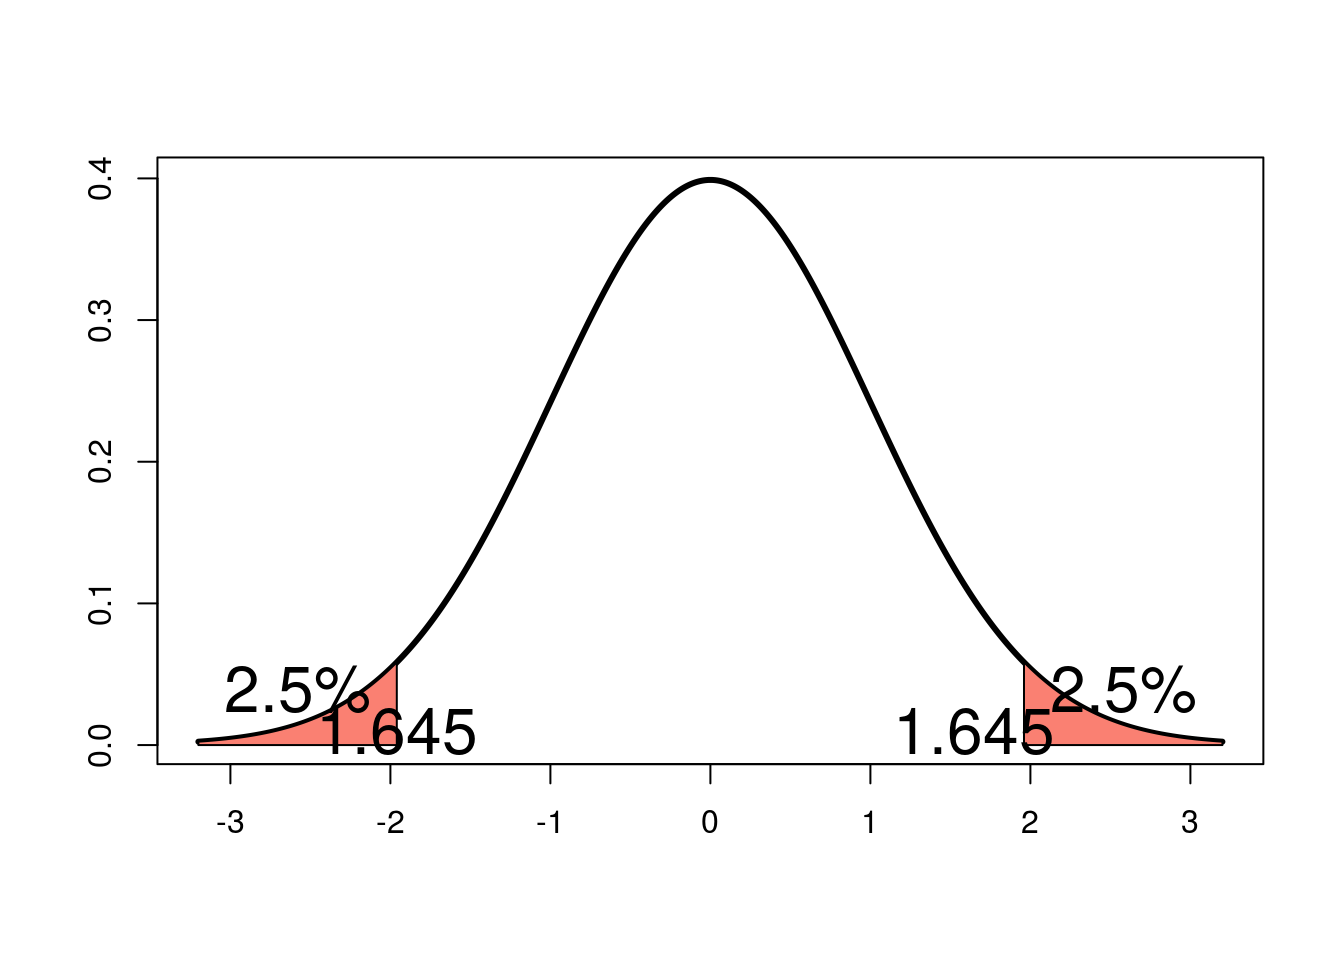
\includegraphics{bioinfBookXIE186_files/figure-latex/unnamed-chunk-68-1.pdf}

\bibliography{packages.bib,book.bib}


\end{document}
